\cleardoublepage
\chapter{Ergebnisse}
\label{results}

\todo[inline]{viel öfter das Wort ``epitaktisch'' und ``Epitaxie'' fallen lassen?}

Unter Nutzung der in Kapitel~\ref{theory} und Kapitel~\ref{models} vorgestellten Methoden werden im folgenden Kapitel Abscheidungssimulationen mit dem Ziel durchgeführt, die Präparation, Durchführung, Möglichkeiten und Einschränkungen des Parsivald-Modelles für PVD und CVD zu prüfen.

Dazu werden in eigenständigen Abschnitten verschiedene Systeme auf unterschiedliche Aspekte untersucht:
Abschnitt~\ref{goldpvd} zeigt anhand von Gold-PVD allgemeine Voruntersuchungen für einen Parametersatz, strukturelle Unterschiede zwischen realen und simulierten Schichten, Schichtabscheidung auf strukturierten Substraten sowie die praktische Skalierbarkeit der Simulation.
Der darauf folgende Abschnitt~\ref{copperpvd} stellt Voruntersuchungen unterschiedlicher Parametersätze, Unebenheiten an der Oberfläche und deren automatische Schließung anhand von Kupfer-PVD dar.
Anschließend werden Kupfer-Nickel-Multilagensysteme in Abschnitt~\ref{multilayer} zur Parsivald-Simulation vorbereitet und mit LAMMPS-simulierten Systemen verglichen.
In Abschnitt~\ref{siliconpvd} werden Silizium-PVD-Systeme mit dem Ziel der Abscheidung amorpher Schichten untersucht.
Zusätzlich werden dort Voruntersuchungen für Siliziumoxid-CVD durchgeführt.
Abschnitt~\ref{aluminaald} kehrt kurz zum Thema der Bachelorarbeit zurück und untersucht TMA und Wasser als Precursoren der \ce{Al2O3}-ALD.
%% Zuletzt werden in Abschnitt~\ref{silicacvd} Precursor-Reaktionen und die darauf basierende Siliziumoxid-CVD behandelt.

\section{Gold-PVD}
\label{goldpvd}

Als Testsystem für PVD-Prozesse bietet sich Gold-PVD an, die zwar durch Oberflächendiffusion dominiert wird, jedoch ideale fcc-kristalline Strukturen bildet.
Die genutzte EAM-Potentialdatei stammt aus dem \todo{ref}LAMMPS-Paket, basiert aber auf Parametern von Foiles et al.\cite{foiles_embedded-atom-method_1986}, die für Einbettung einzelner Atome in Bulk- und Oberflächensysteme optimiert wurden.

\subsection{Voruntersuchungen}

Zur Validierung grundlegender Materialeigenschaften wurden Bindungslängen, Dichten und Koordinationszahlen aus einer relaxierten kristallinen Phase untersucht (Tabelle \ref{tab:goldpreresults}).
Zur Bestimmung dieser Werte wurde ein Goldkristall von \SI{40x40x40}{\angstrom} Größe auf \SI{1000}{\kelvin} aufgeheizt, im kanonischen Ensemble relaxiert und anschließend abgekühlt.
Wie man den Ergebnissen ansehen kann, bleibt die Kristallstruktur erwartungsgemäß erhalten (die Schmelztemperatur wurde für die Relaxierung nicht überschritten) und steht in guter Übereinstimmung mit Literaturwerten.
Die Parametrisierung repräsentiert somit das Zielsystem.

\begin{table}
  %% \oddrowcolors
  \caption[Eigenschaften von Gold]{Vergleich der Eigenschaften von Gold mit experimentellen und Literaturdaten als Voruntersuchung des PVD-Prozesses
    %% \todo[inline]{ref}
  }
  \label{tab:goldpreresults}
  \begin{tabularx}{\textwidth}{|lXXXX|}
    \hline
    \textbf{unters. Größe} & \textbf{Temperatur} & \textbf{Simulation} & \textbf{Experiment} & \textbf{Abweichung}\\
    \hline
    Bindungslänge  &  \SI{50}{\kelvin}   &  \SI{2.885}{\angstrom}                    &  \SI{2.884}{\angstrom}                    &  \SI{0.05}{\percent}  \\
    Koordination   &  \SI{50}{\kelvin}   &  \SI{12.00}{}                             &  \SI{12.00}{}                             &  \SI{0}{\percent}     \\
    Dichte         &  \SI{300}{\kelvin}  &  \SI{18.99}{\gram\per\cubic\centi\meter}  &  \SI{19.30}{\gram\per\cubic\centi\meter}  &  \SI{1.6}{\percent}   \\
    Dichte         &  \SI{500}{\kelvin}  &  \SI{18.89}{\gram\per\cubic\centi\meter}  &  \SI{19.13}{\gram\per\cubic\centi\meter}  &  \SI{1.2}{\percent}   \\
    \hline
  \end{tabularx}
\end{table}

%% \todo[inline]{Oberflächenvalidierung}

\subsection{Thermodynamische Eigenschaften}
\label{goldthermo}

Neben strukturellen Eigenschaften bilden EAM-Potentiale auch einige thermodynamische Eigenschaften von Metallen ab.
Für deren Untersuchung wurde die Massendichte in Abhängigkeit der Temperatur für die Teststruktur aufgenommen, die langsam auf \SI{2000}{\kelvin}, also weit über den Schmelzpunkt von \SI{1337}{\kelvin}, aufgeheizt wurde.
Die Ergebnisse (Abbildung \ref{fig:goldthermo}) zeigen gute Übereinstimmung mit experimentellen Daten, wofür Relaxationszeiten $t_\text{relax}$ oberhalb von \SI{20}{\pico\second} und Thermostat-Dämpfungsparameter $D_T$ \SI{\approx0.02}{\femto\second} als notwendig ermittelt wurden.
Bei geringeren $t_\text{relax}$ oder $D_T$ relaxiert das System innerhalb eines Temperaturschrittes nicht vollständig, wodurch der Schmelzpunkt überschätzt wird, wie in Abbildung \ref{fig:goldthermo-b} zu sehen ist.

\begin{figure}
  \captionsetup[subfigure]{singlelinecheck=false}
  \def\subfigwidth{7cm}
  \begin{subfigure}[t]{\subfigwidth}
    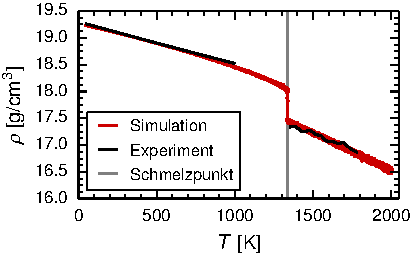
\includegraphics[width=\textwidth]{gold_bestthermo}
    \subcaption{Temperaturverlauf bei $ t_\text{relax}=\SI{50}{\pico\second}$ und $D_T=\SI{0.02}{\femto\second}$}
    \label{fig:goldthermo-a}
  \end{subfigure}
  \hfill
  \begin{subfigure}[t]{\subfigwidth}
    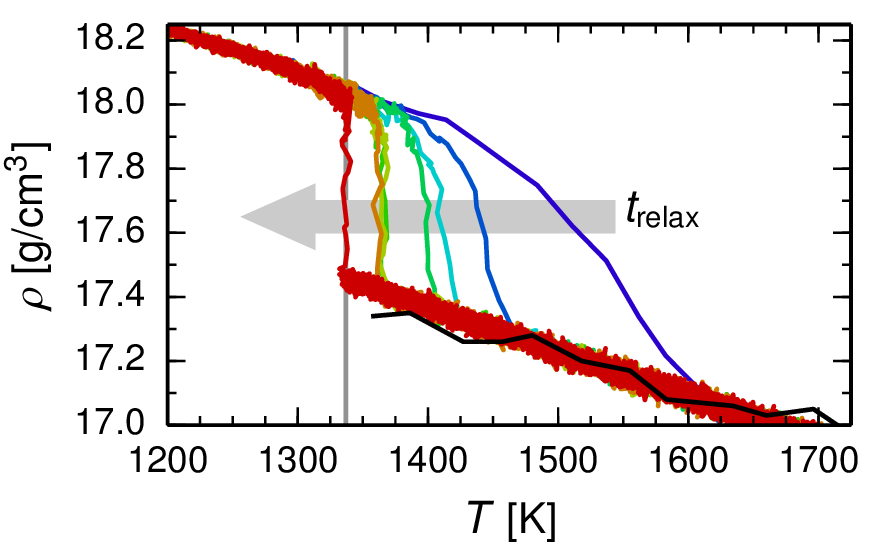
\includegraphics[width=\textwidth]{gold_relaxtime}
    \subcaption{Abhängigkeit des simulierten Schmelzpunktes von der Relaxationszeit}
    \label{fig:goldthermo-b}
  \end{subfigure}
  \caption[Ergebnisse thermodynamischer Simulationen von Gold]{Ergebnisse thermodynamischer Simulationen von Gold.
    Verlauf stimmt gut mit experimentellen Daten (schwarze Linien) überein.
    Experimentelle Werte stammen aus Standardliteratur sowie von Brillo et al.\cite{brillo_density_2006}.
  }
  \label{fig:goldthermo}
\end{figure}

\subsection{Prozess-Simulation}

Zur Simulation eines Gold-PVD-Prozesses mit Parsivald wurden die untersuchten Potentialparameter sowie ein Kristallsubstrat im PVD-Modus eingelesen und Relaxationszeiten und Größen der MD-Simulationsräume aus den Vorbetrachtungen übernommen.
Damit ergeben sich Reaktionsräume der Größe \SI{37x37x25}{\angstrom} mit jeweils ca. \num{1800} Atomen, Relaxationszeiten von \SI{1.4}{\nano\second} in \num{1400} Simulationsschritten und Auftreffgeschwindigkeiten von \SI{4}{\angstrom/\pico\second}, die aus üblichen Sputterbedingungen stammen.\todo{wie berechnet?}

Abbildung \ref{fig:golddepositions-a} zeigt, wie das Substrat unter Erhalt der Kristallstruktur fortgesetzt wird.
Poren und Einschlüsse wurden durch Untersuchung der Alphastruktur nicht gefunden.
Abbildung \ref{fig:goldroughness-a} stellt die Rauheit dar, die beim glatten Substrat über den Abscheidungszeitraum konstant geblieben ist.
Fehler- und Abbruchraten bei den LAMMPS-Berechnungen lagen mit \SI{0.25}{\percent} unterhalb des aus den ALD-Prozessen der Bachelorarbeit erwarteten Wertes von \SI{5}{\percent}

\subsubsection{Wachstum auf strukturierten Substraten}

Neben dem glatten Substrat wurden auch Abscheidungen auf strukturierten Substraten (Abbildung \ref{fig:golddepositions}) mit den gleichbleibenden Prozessbedingungen simuliert.
Als Substrate wurden Stufen oder Spitzen mit einer Höhe von jeweils \SI{20}{\angstrom} und Neigungen von \SI{15}{\degree}, \SI{20}{\degree}, \SI{30}{\degree}, \SI{45}{\degree}, \SI{60}{\degree} und \SI{90}{\degree} präpariert.
Auf vorherige Relaxierung der Substrate wurde aufgrund der Prozessstabilität sowie der relaxierenden Eigenschaften der MD-Ereignisse verzichtet.
Zusätzlich wurden Lamellen und Gitter mit einer Strukturbreite von \SI{16}{\angstrom} zur Untersuchung eventueller Prozessartefakte präpariert.

\begin{figure}
  \captionsetup[subfigure]{singlelinecheck=false}
  \def\subfigwidth{0.31\textwidth}
  \begin{subfigure}[t]{\subfigwidth}
    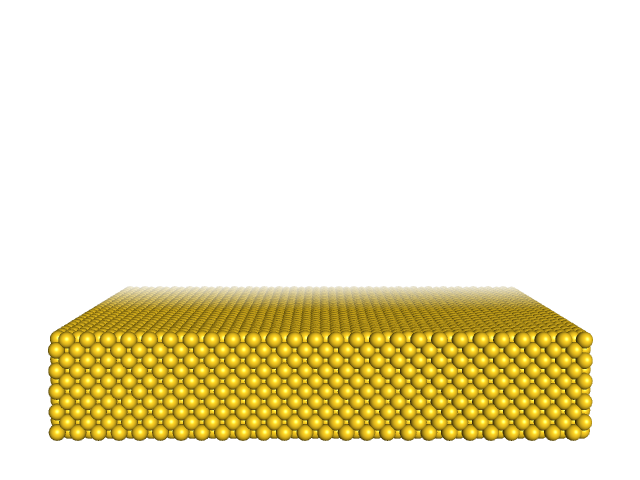
\includegraphics[width=\textwidth]{Au_substrate_flat}
    \subcaption{Glattes Gold-Substrat}
    \label{fig:golddepositions-a}
  \end{subfigure}
  \hfill
  \begin{subfigure}[t]{\subfigwidth}
    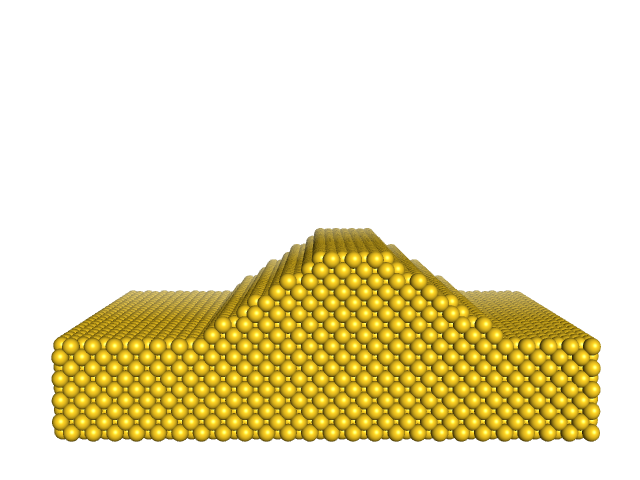
\includegraphics[width=\textwidth]{Au_substrate_step30}
    \subcaption{Gold-Stufe, \SI{30}{\degree}}
    \label{fig:golddepositions-b}
  \end{subfigure}
  \hfill
  \begin{subfigure}[t]{\subfigwidth}
    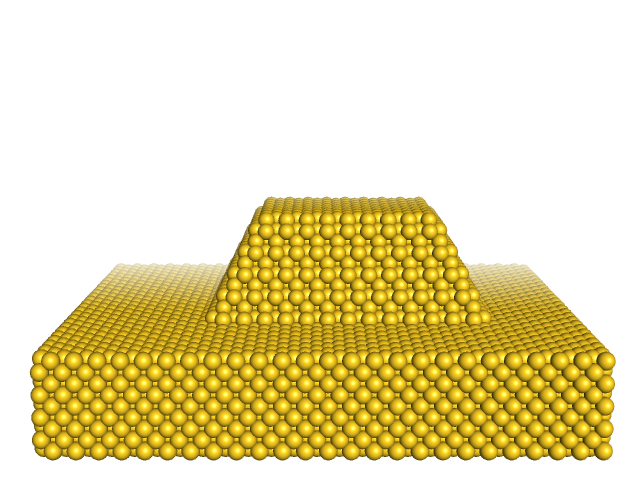
\includegraphics[width=\textwidth]{Au_substrate_tip60}
    \subcaption{Gold-Spitze, \SI{60}{\degree}}
    \label{fig:golddepositions-c}
  \end{subfigure}

  \LARGE\center{$\Downarrow$}
  \vspace{0.25cm}

  \captionsetup[subfigure]{singlelinecheck=false}
  \def\subfigwidth{0.31\textwidth}
  \begin{subfigure}[t]{\subfigwidth}
    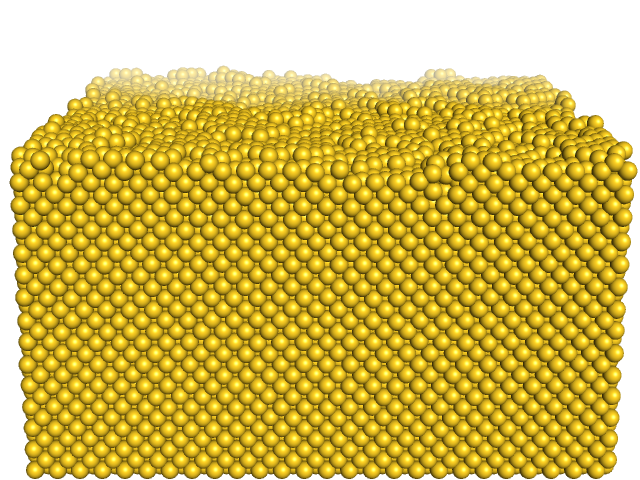
\includegraphics[width=\textwidth]{Au_deposition_flat}
    \subcaption{Glatte, kristalline Schicht ($\sigma_z = \SI{1.2}{\angstrom}$)}
    \label{fig:golddepositions-d}
  \end{subfigure}
  \hfill
  \begin{subfigure}[t]{\subfigwidth}
    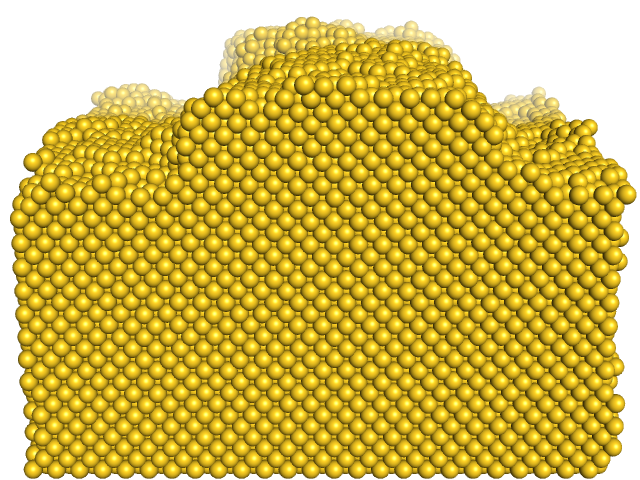
\includegraphics[width=\textwidth]{Au_deposition_step30}
    \subcaption{Fortsetzung der Stufe ($\sigma_z = \SI{6.4}{\angstrom}$)}
    \label{fig:golddepositions-e}
  \end{subfigure}
  \hfill
  \begin{subfigure}[t]{\subfigwidth}
    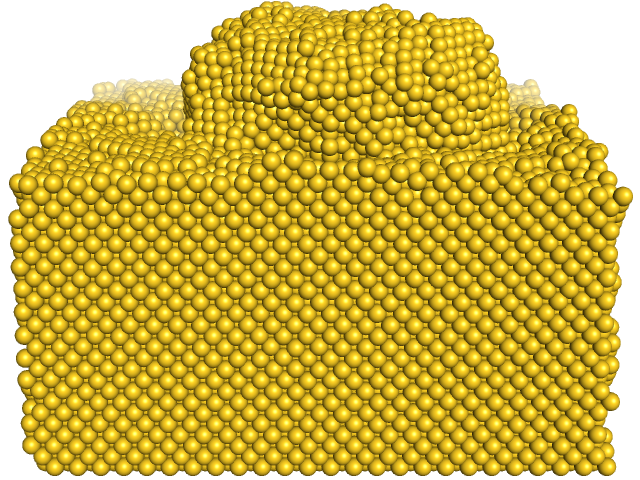
\includegraphics[width=\textwidth]{Au_deposition_tip60}
    \subcaption{Fortsetzung der Spitze ($\sigma_z = \SI{8.0}{\angstrom}$)}
    \label{fig:golddepositions-f}
  \end{subfigure}
  \caption[Gold-Abscheidung auf strukturierten Substraten]{
    Goldschicht nach 50 Abscheidungsschritten (\SI{47}{\angstrom}) auf verschiedenen Substraten
  }
  \label{fig:golddepositions}
\end{figure}

\begin{figure}
  \captionsetup[subfigure]{singlelinecheck=false}
  \def\subfigwidth{0.49\textwidth}

  \begin{subfigure}[t]{\subfigwidth}
    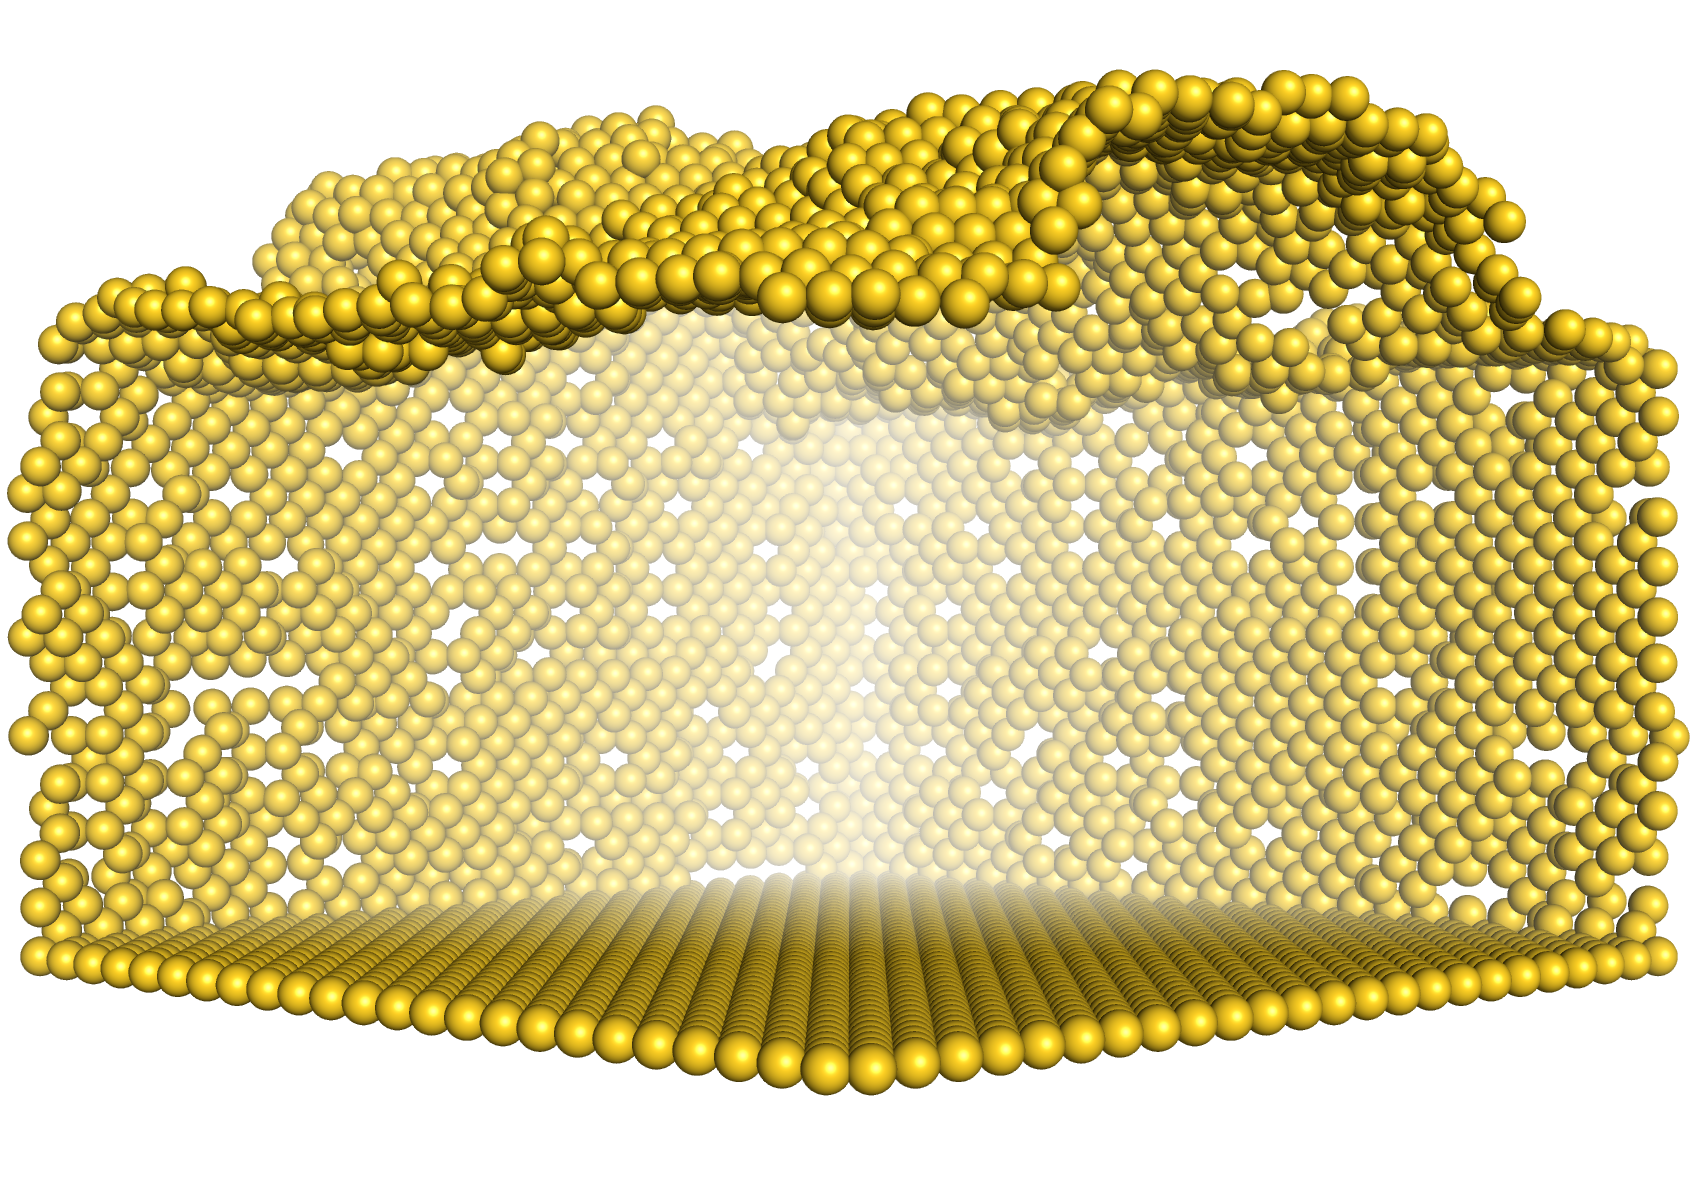
\includegraphics[width=\textwidth]{gold_step30_pockets}
    \subcaption{\SI{30}{\degree}-Stufe: Keine Poren oder Einschlüsse}
    \label{fig:goldpockets-a}
  \end{subfigure}
  \hfill
  \begin{subfigure}[t]{\subfigwidth}
    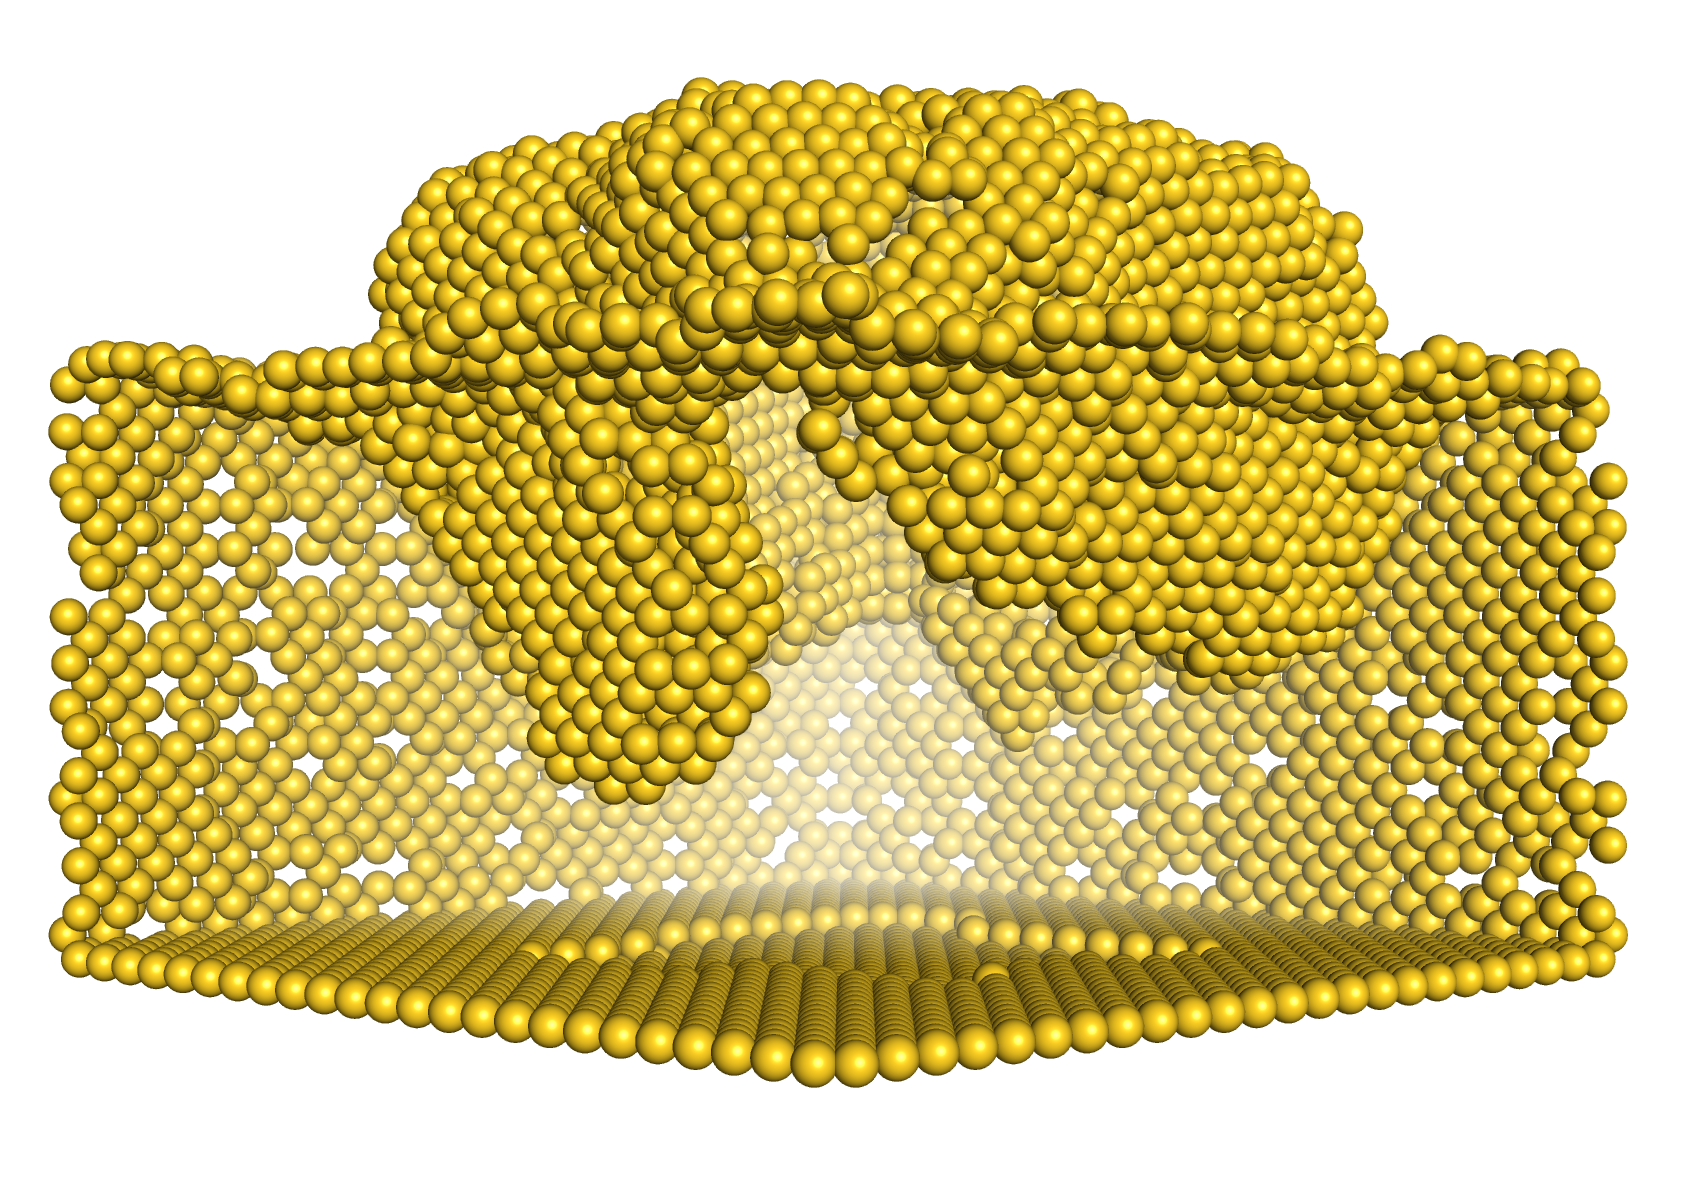
\includegraphics[width=\textwidth]{gold_tip90_pockets}
    \subcaption{Porenbildung an der Basis der \SI{90}{\degree}-Spitze}
    \label{fig:goldpockets-b}
  \end{subfigure}

  \caption[Porenbildung bei Gold-Strukturen]{Porenbildung bei Gold-Strukturen nach 40 Abscheidungsschritten (ca. \num{22000} PVD-Ereignisse $\hat{=}$ \SI{38}{\angstrom}).
  }
  \label{fig:goldpockets}
\end{figure}

Wie man den Alpha-Formen der simulierten Strukturen (Abbildung \ref{fig:goldpockets-a}) entnehmen kann, beinhaltet das abgeschiedene Gold bei geringen Neigungswinkeln keine Kristalldefekte, Poren oder Einschlüsse.
Bei Abscheidungen auf Substrate hoher Neigungswinkel (>\SI{60}{\degree}) bilden sich Poren mit größerer Ausdehnung (>\SI{20}{\angstrom}).
Durch Bildung von Überhängen an den Stufen werden die Poren zu Hohlräumen abgeschlossen, die nicht durch Relaxierung geschlossen werden.
Dies zeigt sich auch in den Oberflächenrauheiten der untersuchten Strukturen (Abbildung \ref{fig:goldroughness}).

\clearpage
\subsection{Vergleich mit gesputterten Schichten}

AFM-Untersuchungen gesputterter Goldschichten zeigen polykristallines Wachstum mit Rauheiten im Bereich von \SI{1.1}{\nano\meter} (etwa drei fcc-Kristallschichten)\cite{svorcik_annealing_2011}.
Dabei wird die Oberflächenrauheit von der Bildung von Nanopartikeln dominiert, deren Schmelztemperaturen mit der Größe der Partikel zunehmen\cite{liu_melting_2001}.
Kleinere Goldpartikeln verschmelzen oberhalb ihrer spezifischen Schmelztemperatur zu größeren Partikeln, wodurch die Rauheit der Goldoberfläche mit höheren Substrat- oder Annealing-Temperaturen zunimmt.
Bei \todo{Vergleich womit?}vergleichsweise niedrigen Temperaturen, wie sie bei Sputtering vorhanden sind, werden durch Unterbindung der Verschmelzung kleiner Goldpartikel geringere Rauheiten erreicht, die mit längerer Sputterdauer weiter abnehmen\cite{svorcik_annealing_2011}.

In Parsivald-Simulationen ist dieser Trend bisher nur selten zu beobachten, wie etwa bei der \SI{45}{\degree}-Spitze, deren Rauheit gegen Ende der Simulation langsam abnimmt.
Die Systeme wachsen in monokristallinen Schichten entlang der Kristallebenen, jedoch zeigen Abscheidungssimulationen auf einigen strukturierten Substraten zusätzliche Porenbildung an Überhängen, die in der aktuellen Oberflächensuche begründet sind.
So wird die Oberfläche und damit mögliche Ereignisorte parallel zur Z-Achse gesucht, anstatt die Alpha-Form über eine Delaunay-Triangulation der Atompositionen zu ermitteln, wie es zur bereits Auswertung der simulierten Strukturen durchgeführt wird.
Somit werden höher gelegene Ereignisorte in der direkten Nachbarschaft bevorzugt, was sich in der Verstärkung von Überhängen bei strukturierten Substraten mit hohen Neigungswinkeln zeigt (Abbildung \ref{fig:goldpockets-b}).
Als Lösung bieten sich die eben genannten Alpha-Formen an, welche jedoch erst für das Parsivald-Modell optimiert werden müssen (Abschnitt \ref{datadelaunay}).

Bei der Analyse der simulierten Strukturen wurde bei Abscheidungen auf glatten Substraten eine Rauheit von \SI{0.12}{\nano\meter} ermittelt, welche nur ca. \SI{10}{\percent} der experimentellen Werte beziehungsweise einer Lage von Goldatomen entspricht.
Strukturierte Substrate zeigen hier höhere Rauheiten, die zwar den experimentell bestimmten Rauheiten entsprechen (Abbildung \ref{fig:goldroughness}), aber ebenfalls keine Nanopartikel enthalten, sondern aus monokristallinen Schichten bestehen.
Daran lässt sich erkennen, dass die verwendeten \todo{word}MD-Simulation-Boxen zu klein und die Relaxationszeiten zu kurz sind, um die Bildung von Nanopartikeln darstellen zu können.
Zusätzlich verhindern kleine MD-Boxen in Verbindung mit monokristallinen Substraten die Ausbildung polykristalliner Strukturen, was sich im Wachstum monokristalliner Schichten äußert.
Derartige Finite-Size-Effekte sind Molekulardynamik-Simulationen inhärent, werden jedoch durch Parsivald für einige Systeme zusätzlich verstärkt.
Bei Abscheidung amorpher Schichten, wie für CVD- und ALD-Prozesse üblich, konnte dieser Effekt bisher nicht beobachtet werden (Abschnitt \ref{siliconpvd}).

\begin{figure}
  \captionsetup[subfigure]{singlelinecheck=false}
  \def\subfigwidth{0.49\textwidth}

  \begin{subfigure}[t]{\subfigwidth}
    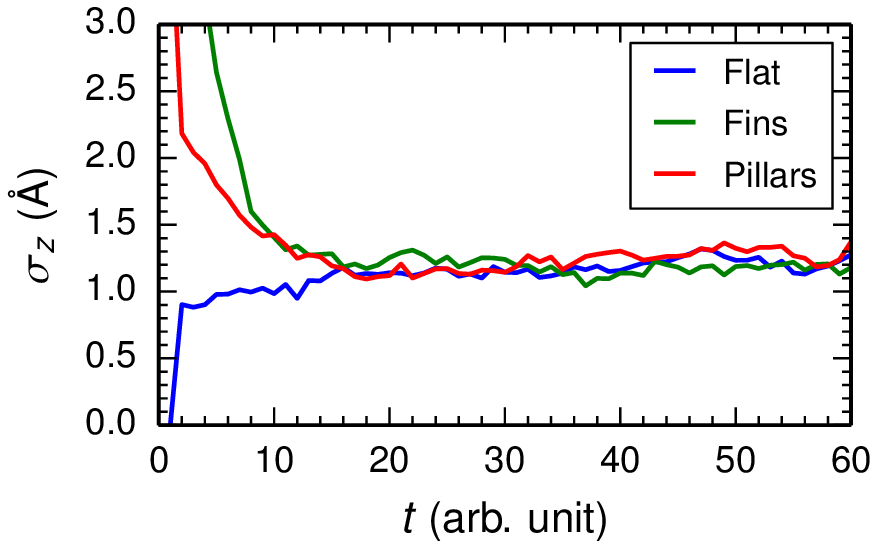
\includegraphics[width=\textwidth]{gold_goodroughness}
    \subcaption{Zeitverlauf der Rauheit von glatten (Flat) und fein strukturierten Oberflächen (Fins, Pillars: \SI{10}{\angstrom} breite Erhebungen)}
    \label{fig:goldroughness-a}
  \end{subfigure}
  \hfill
  \begin{subfigure}[t]{\subfigwidth}
    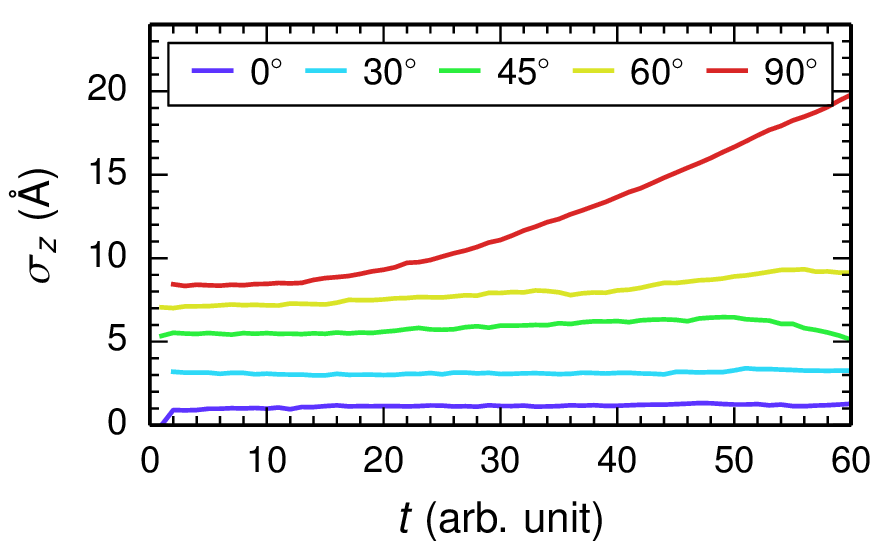
\includegraphics[width=\textwidth]{gold_tiproughness}
    \subcaption{Zeitverlauf der Rauheit von \SI{50}{\angstrom} breiten Spitzen variabler Steigung.
      Oberflächenrauheiten werden nicht verringert
    }
    \label{fig:goldroughness-b}
  \end{subfigure}

  \caption[Oberflächenrauheit von Gold]{Oberflächenrauheit von Gold.
    Im idealen Fall konvergiert die Rauheit gegen einen konstanten Wert von \SI{1.2}{\angstrom}
  }
  \label{fig:goldroughness}

\end{figure}

\subsection{Skalierbarkeit mit der Simulationsgröße}

Die Größe der simulierten Strukturen, wie sie beispielsweise für Beschichtungen kompletter \todo{Nanodevice}Nano-Bauelemente von Interesse sind, ist bei jeder Simulationsmethode durch verschiedene Einflüsse wie Speicherbedarf und Laufzeit limitiert.
Allgemein lässt sich sagen, dass präzisere Methoden nur auf kleineren Systemen und kürzeren Zeitskalen funktionieren (Abbildung \ref{fig:methodscales}).
Atomistische Methoden, insbesondere die Molekulardynamik, sind von theoretischer Seite durch die Notwendigkeit der paarweisen Interaktionen und von technischer Seite durch Speicher- und Netzwerkbandbreite begrenzt.
Somit sind Systeme mit mehr als \num{100000} Atomen nur mit hohem Aufwand über viele Zeitschritte hinweg berechenbar.
Die in Abschnitt \ref{datastructures} vorgestellten Überlegungen zur Optimierung, in Kombination mit dem Parallelisierungsansatz des Parsivald-Modelles aus Abschnitt \ref{parsivald}, sollen hier einem praktischen Test unterzogen werden.

Dazu werden verschiedene quadratische Substrate mit Breiten von \SI{100}{\angstrom}, \SI{200}{\angstrom}, \SI{500}{\angstrom}, \SI{1000}{\angstrom} und \SI{10000}{\angstrom} und \SI{20000}{\angstrom} auf Speicherbedarf, Laufzeit, Anzahl der Atome und Ereignisse, Zahl gleichzeitig aktiver Worker und Bedeckungsgrad der Oberfläche mit aktiven Ereignissen untersucht (Tabelle \ref{tab:goldscalability}).

\begin{table}\begin{threeparttable}

    \caption[asd]{Untersuchungen zur Skalierbarkeit des Systemes}
    \label{tab:goldscalability}

    \begin{tabularx}{\textwidth}{|Xrrrrrrr|}
      \hline
      \textbf{Größe}\tnote{2}  &  \textbf{Wachst.}     &  \textbf{Atome}  &  \textbf{Ereignisse}  &  \textbf{Worker}\tnote{a}  ~            &  \textbf{Bed.}\tnote{e}  &  \textbf{Laufzeit}  &  \textbf{RAM}\tnote{f}  \\
      \hline
      \SI{106}{\angstrom}      &  \SI{70}{\angstrom}   &  \num{59549}     &  \num{46030}          &  \num{1.8}\tnote{b}        (\num{4})    &  \SI{21.9}{\percent}     &  \SI{32.2}{\hour}   &  \SI{254}{\mebi\byte}   \\
      \SI{204}{\angstrom}      &  \SI{42}{\angstrom}   &  \num{152374}    &  \num{102374}         &  \num{14.5}\tnote{b}       (\num{18})   &  \SI{47.7}{\percent}     &  \SI{25.5}{\hour}   &  ~                      \\
      \SI{204}{\angstrom}      &  \SI{42}{\angstrom}   &  \num{152374}    &  \num{102374}         &  \num{14.5}\tnote{b}       (\num{18})   &  \SI{47.7}{\percent}     &  \SI{25.5}{\hour}   &  \SI{257}{\mebi\byte}   \\
      \SI{500}{\angstrom}      &  \SI{93}{\angstrom}   &  \num{1708600}   &  \num{1401081}        &  \num{24.8}                (\num{50})   &  \SI{13.6}{\percent}     &  \SI{73.6}{\hour}   &  \SI{282}{\mebi\byte}   \\
      \SI{1000}{\angstrom}     &  \SI{5.4}{\angstrom}  &  \num{1591908}   &  \num{381588}         &  \num{44.8}                (\num{46})   &  \SI{6.1}{\percent}      &  \SI{1.5}{\hour}    &  \SI{368}{\mebi\byte}   \\
      \SI{1000}{\angstrom}     &  ~                    &  \num{6733948}   &  \num{5539942}        &  \num{75.4}                (\num{149})  &  \SI{10.3}{\percent}     &  \SI{97.5}{\hour}   &  ~                      \\
      \SI{1}{\micro\meter}     &  \SI{1.3}{\angstrom}  &  \num{1.3e8}     &  \num{8186990}        &  \num{25.4}\tnote{c}       (\num{46})   &  \SI{0.03}{\percent}     &  \SI{117.5}{\hour}  &  \SI{11.5}{\gibi\byte}  \\
      \SI{2}{\micro\meter}     &  \SI{0.4}{\angstrom}  &  \num{4.9e8}     &  \num{10356031}       &  \num{26.3}\tnote{c}       (\num{46})   &  \SI{0.009}{\percent}    &  \SI{117.5}{\hour}  &  ~                      \\
      \SI{2}{\micro\meter}     &  \SI{1.0}{\angstrom}  &  \num{5.1e8}     &  \num{25855695}       &  \num{189}\tnote{d}        (\num{245})  &  \SI{0.06}{\percent}     &  \SI{186.8}{\hour}  &  \SI{45.4}{\gibi\byte}  \\
      \SI{4}{\micro\meter}     &  ~                    &  \num{1.9e9}     &  ~                    &  ~                         ~            &  ~                       &  ~                  &  \SI{182}{\gibi\byte}   \\
      \hline
    \end{tabularx}

    \begin{tablenotes}
    \item[2] Breite der quadratischen Oberfläche
    \item[a] Mittelwert und Maximum der zeitgleich bearbeiteten Ereignisse
    \item[b] Maximale Ereignisdichte erreicht.
      Restliche Worker sind im Wartezustand.
    \item[c] Inzwischen behobener Fehler im Host-Code hat Workerneustart verhindert
    \item[d] Maximale Bandbreite des Hosts erreicht.
      Längere MD-Simulationen erlauben mehr Worker.
    \item[e] Bedeckung: Anteil der von laufenden Ereignissen abgedeckten Oberfläche
    \item[f] Vom Hostprozess verbrauchten
    \end{tablenotes}

\end{threeparttable}\end{table}

Mit \SI{94}{\byte} pro Atom, zusätzlich zum konstanten Programmspeicher von \SI{253}{\mebi\byte}, können auch extreme Simulationsräume mit 2 Milliarden Atomen auf einer Oberfläche von \SI{4x4}{\micro\meter} vom Arbeitsspeicher moderner Hochleistungsrechner verwaltet werden können.

Anders sieht es bei der notwendigen Rechenleistung aus:
Während kleine Simulationsräume (\SI{<200}{\angstrom}) nicht wesentlich von der parallelen Rechenleistung profitieren können, scheitern größere Prozesse am Mangel daran:
Im zweiten Test mit einer \SI{2x2}{\micro\meter} großen Struktur wurde die Grenze der Bandbreite des Hostprozesses erreicht:
Die Tests haben gezeigt, dass dieser \num{38.4} Ereignisse pro Sekunde vorbereiten, starten und auswerten kann.
Mit \SI{4.86}{\second} Laufzeit pro Gold-PVD-Ereignis kann der Hostprozess aber nur 189 parallele Worker dauerhaft mit Ereignissen versorgen.
Die eigentliche Beschränkung liegt folglich in der genutzten Potentialart:
Kompliziertere und damit langsamere Potentiale, wie die später genutzten ReaxFF-Potentiale, benötigen meist mehr als \SI{30}{\second} für ein Ereignis, in extremen Fällen sogar \SI{5}{\minute}.
Somit erlauben sie theoretisch \num{1152} beziehungsweise \num{11520} parallele Worker und übersteigen damit die Möglichkeit dessen, was einem einzelnen Nutzer an einem Hochleistungsrechencluster zur Verfügung steht.
Leider erhöht sich damit auch die insgesamt benötigte Rechenzeit linear.

Die verbleibende Einschränkung wird somit von den verfügbaren Rechenkernen gebildet.
In Simulationen mit Substratgrößen auf der Mikrometer-Skala wurden nur kleine Teile der Oberfläche (\SI{<0.1}{\percent}) zeitgleich von Ereignissen simuliert.
Bei Oberflächen von \SI{2x2}{\micro\meter} Größe sind in dichtester Packung der MD-Boxen mit je \SI{37x37}{\angstrom} Größe maximal \num{291600} parallele Ereignisse möglich.
Tatsächlich werden aufgrund der Überdeckung der Ereignisse durch die zufällige Wahl der Reaktionsorte häufig \SI{<40}{\percent} davon zeitgleich simuliert.
Dennoch liegt die Zahl der verfügbaren Prozessorkerne um Größenordnungen unterhalb des optimalen Wertes, was sich in langen Simulationslaufzeiten äußert (\SI{186.8}{\hour} für \SI{1.0}{\angstrom}).

Zusammenfassend lässt sich sagen, dass Systeme mit einer Größe zwischen \SI{50x50}{\nano\meter} und \SI{300x300}{\nano\meter} mit modernen Computerclustern effizient berechenbar sind, wo hingegen kleinere Systeme nicht signifikant von der Effizienzsteigerung profitieren können und für größere Systeme die notwendige Rechenleistung unerreichbar bleibt.


\clearpage
\section{Kupfer-PVD}
\label{copperpvd}

Ein zweites PVD-System stellt Kupfer dar, wofür eine Vielzahl an unterschiedlichen Parametrisierungen vorliegen (Tabelle \ref{tab:copperpots}).
Es stellt sich die Aufgabe, eine passende Parametrisierung darunter zu suchen und zu entscheiden, inwiefern eine Vorauswahl anhand weniger Parameter \todo{chword} sinnvoll ist.
Kupfer bildet ebenfalls fcc-Kristalle, 

\begin{table}[hbtp]
  \caption[EAM-Parametrisierungen für Kupfersysteme]{EAM-Parametrisierungen für Kupfersysteme.}
  \label{tab:copperpots}
  \rowcolors{0}{white}{lightgray}
  \begin{tabularx}{\textwidth}{|lXc|}
    \hline
    \textbf{Bezeichnung} & \textbf{Anwendung \& Kommentare} & \textbf{Ref.} \\
    \hline
    CuAg.eam.alloy & Strukturelle und thermische Eigenschaften von \ce{Cu-Al} & \cite{williams_embedded-atom_2006} \\
    cu\_ag\_ymwu.eam.alloy & Mono-, Di-, Trimere und Inseln von \ce{Cu} auf \ce{Ag} & \cite{wu_cu/ag_2009} \\
    Cu\_smf7.eam & Oberflächen von \ce{Ni-Cu}-Legierungen bei \SI{800}{\kelvin} & \cite{foiles_calculation_1985} \\
    Cu\_u3.eam & Oberflächen und Bulks verschiedener Legierungen & \cite{foiles_embedded-atom-method_1986} \\
    Cu\_u6.eam & Aktivierungsenergie für Eigendiffusionen & \cite{adams_self-diffusion_1989} \\
    Cu-Zr\_2.eam.fs & Flüssige und amorphe \ce{Cu-Zr}-Legierungen & \cite{mendelev_development_2009} \\
    Cu-Zr.eam.fs & Flüssige und amorphe \ce{Cu-Zr}-Legierungen & \cite{mendelev_using_2007} \\
    Mendelev\_Cu2\_2012.eam.fs & Unterkühlte \ce{Al-Cu}-Schmelzen. Basiert auf \cite{mendelev_analysis_2008} & \cite{_interatomic_2014} \\
    \hline
  \end{tabularx}
  
\end{table}

\subsection{Voruntersuchungen}

Bei den Voruntersuchungen der strukturellen Eigenschaften konnten einige Parametersätze von LAMMPS nicht akzeptiert werden oder haben sich mit kryptischen Fehlern auf negative Speicherallokierungen aufgehangen.
Die Ergebnisse der drei verbliebenen Potentiale sind jedoch in guter Übereinstimmung mit Literaturwerten (Tabelle \ref{tab:copperpreresults}).
\todo{Dichte}Der Schmelzpunkt wurde jedoch nicht zuverlässig simuliert (Abbildung \ref{fig:copperthermo}).

\begin{table}[hbtp]
  %% \rowcolors{0}{white}{lightgray} 
  \caption[Eigenschaften von Gold]{Vergleich der Eigenschaften von Gold mit experimentellen und Literaturdaten als Voruntersuchung des PVD-Prozesses\todo[inline]{ref}}
  \label{tab:goldpreresults}
  \begin{tabularx}{\textwidth}{|lXXXX|}
    \hline
    \textbf{unters. Größe} & \textbf{Experiment} & \textbf{Cu\_smf7.eam} & \textbf{Cu\_u3.eam} & \textbf{Cu\_u6.eam} \\
    \hline
    Bindungslänge  &  \SI{2.556}{\angstrom} & \SI{2.558}{\angstrom} & \SI{2.558}{\angstrom} & \SI{2.558}{\angstrom} \\
    Koordination   &  \SI{12.00}{} & \SI{12.00}{} & \SI{12.00}{} & \SI{12.00}{} \\
    Dichte         & \SI{8.92}{\gram\per\cubic\centi\meter} & \SI{8.908}{\gram\per\cubic\centi\meter} & \SI{8.915}{\gram\per\cubic\centi\meter} & \SI{8.910}{\gram\per\cubic\centi\meter} \\
    \hline
  \end{tabularx}
\end{table}

\todo[inline]{Oberflächenvalidierung?}

\begin{figure}[tbp]
  \centering
  \captionsetup[subfigure]{singlelinecheck=false}
  \def\subfigwidth{7cm}
  \begin{subfigure}[t]{\subfigwidth}
    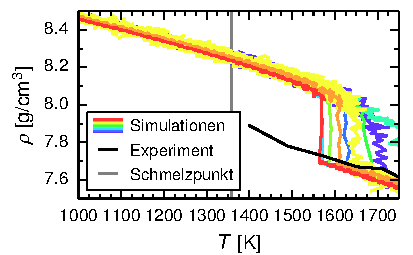
\includegraphics[width=\textwidth]{Cu_u6_meltingpoint}
    \subcaption{Phasenübergang mit Cu\_u6.eam bei unterschiedlichen $t_\text{relax}$}
  \end{subfigure}
  \hfill
  \begin{subfigure}[t]{\subfigwidth}
    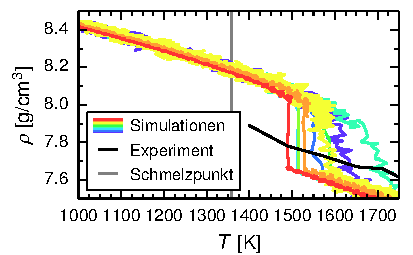
\includegraphics[width=\textwidth]{Cu_smf7_meltingpoint}
    \subcaption{Phasenübergang mit Cu\_smf7.eam bei unterschiedlichen $t_\text{relax}$}
  \end{subfigure}
  \caption[Abweichung der Schmelztemperaturen bei Kupfer-MD]{
    Abweichung der Schmelztemperatur mit verschiedenen Parametrisierungen.
    Experimentelle Werte von Brillo et al.\cite{brillo_density_2006}.
  }
  \label{fig:goldthermo}
\end{figure}

\subsection{Prozess-Simulation}

Äquivalent zur Vorgehensweise beim Gold-PVD-Prozess wurde ein Kupfer-PVD-Prozess gestartet
Zur Simulation eines Gold-PVD-Prozesses mit Parsivald wurden die untersuchten Potentialparameter sowie ein Kristallsubstrat eingelesen, ein Abscheidungsmodus mit zufälligen Auftreffpositionen in der xy-Ebene gewählt und Relaxationszeiten und Reaktionsnachbarschaftsgrößen gewählt, die in den vorheringen Tests als hinreichend ermittelt wurden.
Damit ergaben sich Reaktionsräume der Größe \SI{37x37x25}{\angstrom} mit jeweils ca. 1800 Atomen, Relaxationszeiten von \SI{1.4}{\nano\second} in \SI{1400}{} Simulationsschritten und Auftreffgeschwindigkeiten von \SI{4}{\angstrom/\pico\second}, die aus üblichen Sputterbedingungen stammen.\todo{wie berechnet?}
Die \SI{100x100}{\angstrom} breiten Kristalle werden perfekt fortgesetzt, wobei nach 10 Kristallschichten eine Rauheit von einem Atomdurchmesser vorliegt, was Übereinstimmung mit einem diffusionsdominierten Abscheidungsprozess zeigt.

\subsubsection{Strukturierte Substrate}

Als Stabilitätsprüfung wurden auch Abscheidungen auf strukturierten Substraten (Abbildung \ref{fig:coppersubstrate}) mit den gleichbleibenden Prozessbedingungen simuliert.
Es wurden Stufen und Spitzen mit Neigungen von jeweils \SI{15}{\degree}, \SI{20}{\degree}, \SI{30}{\degree}, \SI{45}{\degree}, \SI{60}{\degree} und \SI{90}{\degree} bei oben genannten Prozessbedingungen untersucht.
\todo{vorherige Relaxation?}

\begin{figure}[bt]
  \captionsetup[subfigure]{singlelinecheck=false}
  \def\subfigwidth{0.31\textwidth}
  \begin{subfigure}[t]{\subfigwidth}
    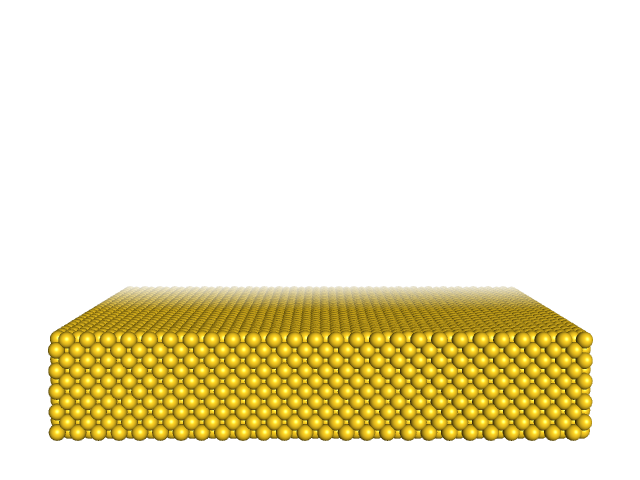
\includegraphics[width=\textwidth]{Au_substrate_flat}
    \subcaption{Glattes Gold-Substrat}
    \label{fig:coppersubstrate-a}
  \end{subfigure}
  \hfill
  \begin{subfigure}[t]{\subfigwidth}
    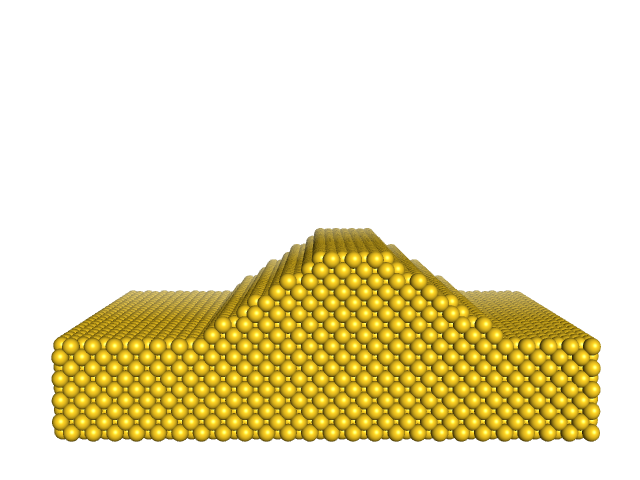
\includegraphics[width=\textwidth]{Au_substrate_step30}
    \subcaption{Gold-Stufe, \SI{30}{\degree}}
    \label{fig:coppersubstrate-b}
  \end{subfigure}
  \hfill
  \begin{subfigure}[t]{\subfigwidth}
    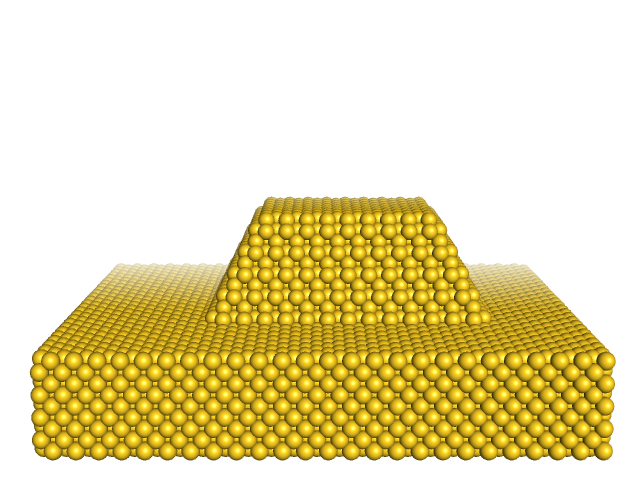
\includegraphics[width=\textwidth]{Au_substrate_tip60}
    \subcaption{Gold-Spitze, \SI{60}{\degree}}
    \label{fig:coppersubstrate-c}
  \end{subfigure}
  \caption[Strukturierte Coppersubstrate]{Coppersubstrate mit unterschiedlicher Struktur und Breite und Tiefe von \SI{100}{\angstrom}.
    Abscheidungen wurden auf glatten Substraten, Stufen und Spitzen vorgenommen.}
  \label{fig:coppersubstrate}
\end{figure}

\begin{figure}[bt]
  \captionsetup[subfigure]{singlelinecheck=false}
  \def\subfigwidth{0.31\textwidth}
  \begin{subfigure}[t]{\subfigwidth}
    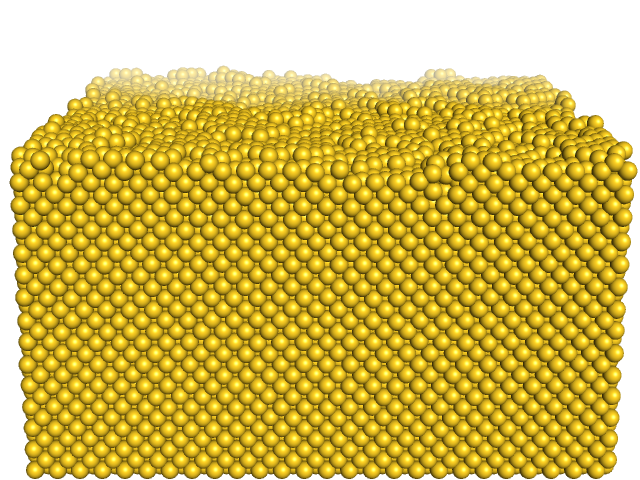
\includegraphics[width=\textwidth]{Au_deposition_flat}
    \subcaption{Abscheidung auf glattem Gold-Substrat}
    \label{fig:copperdepositions-a}
  \end{subfigure}
  \hfill
  \begin{subfigure}[t]{\subfigwidth}
    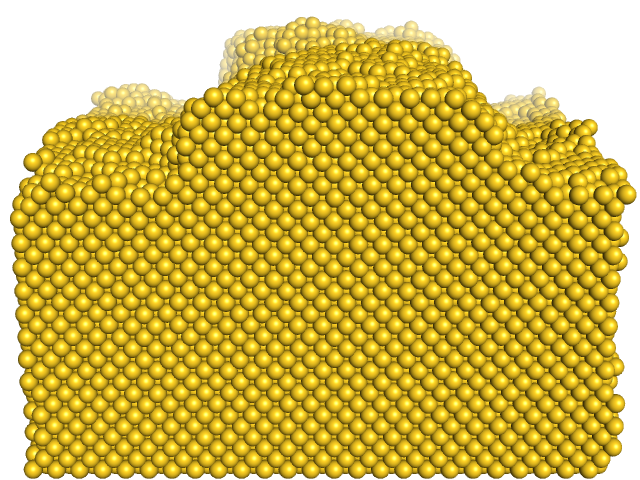
\includegraphics[width=\textwidth]{Au_deposition_step30}
    \subcaption{Abscheidung auf Gold-Stufe, \SI{30}{\degree}}
    \label{fig:copperdepositions-b}
  \end{subfigure}
  \hfill
  \begin{subfigure}[t]{\subfigwidth}
    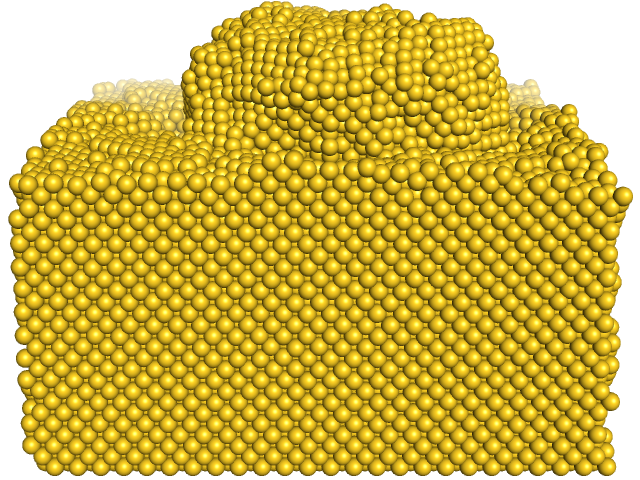
\includegraphics[width=\textwidth]{Au_deposition_tip60}
    \subcaption{Abscheidung auf Gold-Spitze, \SI{60}{\degree}}
    \label{fig:copperdepositions-c}
  \end{subfigure}
  \caption[Abscheidung auf strukturierten Substraten]{
    Ergebnis der Abscheidung.
    Die Substratstruktur bleibt erkennbar, wird aber nach oben verstärkt, ansonsten aber kristallin und glatt fortgesetzt.
  }
  \label{fig:copperdepositions}
\end{figure}

Das Kristallsubstrat wird auch hier fortgesetzt, jedoch verstärken sich Neigungswinkel an Stufen und Spitzen zunehmend.
Nach längeren Laufzeiten entstehen somit Überhänge, die durch Abschluss von unten zu Hohlräumen innerhalb der Struktur führen, welche in der Realität durch thermische Relaxation geschlossen würden.
Dahinter steht einerseits die Notwendigkeit, Gold-Atome bei Ankunft auf der Oberfläche ausreichend diffundieren zu lassen, was beim aktuellen Modell nur innerhalb der Reaktionsraumgrenzen geschieht.

Andererseits liegt ein methodischer Fehler bei Nutzung von Binning-Methoden vor:
Die Oberfläche wird aus algorithmischen Gründen nur entlang der z-Achse bestimmt, woraufhin das neue Atom oberhalb eines Referenzatomes auf der Oberfläche platziert wird.
An Stufen und Kanten werden hierbei höhere Reaktionsorte bevorzugt, an denen das Atom mit \todo{phrasing}statistischer Wahrscheinlichkeit verbleibt.

Einen Lösungsansatz stellt die ausführliche Parametrisierung der Oberfläche dar, beispielsweise per Alpha-Form (siehe Abschnitt \ref{dataalphaform}, über die man die Ereigniswahrscheinlichkeit entsprechend der Einbettungsenergie variierte, angenähert über die Oberflächenkrümmung.

\clearpage
\section{Multilagen-PVD}
\label{multilayer}

Mit PVD-Methoden können auch mehrlagige Schichten abgeschieden werden, die im folgenden Kapitel am Beispiel von dünnen Cu/Ni-Multilagen näher untersucht werden sollen.
Das Kupfer-Nickel-System wurde aufgrund ähnlicher Gitterkonstanten gewählt (Ni:~\SI{3.52}{\angstrom}, Cu:~\SI{3.61}{\angstrom}), die kristallines Wachstum ermöglichen und somit Fehlstellen unterbinden.
Durch die Ähnlichkeit zur Kupfer-PVD kann man zudem auf den dort entwickelten Prozessparametern und den untersuchten Potentialparametersätzen aufbauen.

Im Experiment werden mehrlagige Kupfer-Nickel-Schichten per Elektro\-deposition\cite{yang_pulsed_1995} oder durch Sputtern\cite{cammarata_nanoindentation_1990} hergestellt, wobei üblicherweise Lagendicken im Bereich mehrerer Nanometer erzielt werden.
Dieses Vorgehen lässt sich direkt in Parsivald-Simulationen übertragen, in denen zugunsten der Rechenzeit in den folgenden Untersuchungen vergleichsweise dünne Lagen mit einer Dicke von \SI{1}{\nano\meter} abgeschieden wurden.
Anschließend werden diese auf Ähnlichkeit mit LAMMPS-präparierten Multilagen hinsichtlich ihrer Lagendicke und -rauheit untersucht.
Eine Auswertung der relativen Verteilung der Spezies entlang der Abscheidungsrichtung wird ergänzend für verschiedene Relaxationszeiten als Maß der Lagenqualität durchgeführt.
Abscheidungen von Lagen mit einer Dicke von \SI{6}{\nano\meter} wurden ebenfalls mit Parsivald simuliert, doch mangels verfügbarer Rechenzeit für vergleichbare LAMMPS-Simulationen nicht eingehender untersucht.

Wie bei den Gold-PVD-Simulation zuvor müssen für erfolgreiche Simulationen einige Prozessparameter wie Relaxationszeit, Thermostatdämpfung und Substrattemperatur optimiert werden.
Als Zielgrößen für die Optimierung wurden zur Vermeidung von Fehlstellen die Rauheit der Oberfläche und die Qualität der einzelnen Lagen im Vergleich mit ähnlichen Untersuchungen\cite{zhou_atomistic_1998} gewählt.
In diesen Untersuchungen wurde bereits gezeigt, dass die kinetische Energie der einfallenden Atome einen erheblichen Einfluss auf die Qualität der einzelnen Lagen hat, weshalb gleichartige Untersuchungen nur hinsichtlich der Substrattemperatur durchgeführt wurden.

\subsection{Ergebnisse}

Parsivald-Simulationen erzeugen nach korrekter Parametereinstellung monokristallin gewachsene, klar abgegrenzte Atomlagen geringer Rauheit, die sich gut mit den Ergebnissen gleichartiger LAMMPS-Simulationen decken (Abbildung~\ref{fig:multilayerresults}).
RMS-Rauheiten um \SI{1.2}{\angstrom} stellen sich mit beiden Simulationsmethoden bis zur zehnten Lage ein und stimmen somit miteinander und mit den bisherigen Ergebnissen überein (Abbildung~\ref{fig:multilayerplots-a}).

Zuvor war eine Anpassung der Temperaturen und Relaxationszeiten notwendig, die jedoch für LAMMPS und Parsivald gleichermaßen gelten.
Als Richtwert wurde die Qualität der einzelnen Lagen in Form des Anteils der Spezies in Abhängigkeit der Höhe über dem Substrat genutzt (Abbildung~\ref{fig:multilayerplots-b}).
Lagen schlechterer Qualität zeigen eine höhere Durchmischung der Schichten, was wiederum zu einer Senkung der relativen Häufigkeit einer Spezies innerhalb ihrer Schicht führt, wie man für die beiden Verteilungen bei einer Relaxationszeit von \SI{0.2}{\femto\second} pro Ereignis beobachten kann.
Erst bei Verdopplung der Relaxationszeit bilden sich klar abgegrenzte Lagen aus, wie sie in Abbildung~\ref{fig:multilayerresults} dargestellt sind.

In Anhang~\ref{appendix:multilayer} ist eine Auswahl von mehrlagigen Kupfer-Nickel-Schichten dargestellt, die durch Unterrelaxation verursachte strukturelle Fehler aufweisen.
Bei größeren Systemen ist zudem mit Verspannungen aufgrund der unterschiedlichen Bindungslängen Gitterversetzungen und Fehlstellen zu rechnen, die allerdings durch Finite-Size-Effekte unterdrückt sein können.

\begin{figure}
  \captionsetup[subfigure]{singlelinecheck=false}
  \def\subfigwidth{7cm}
  \begin{subfigure}[t]{\subfigwidth}
    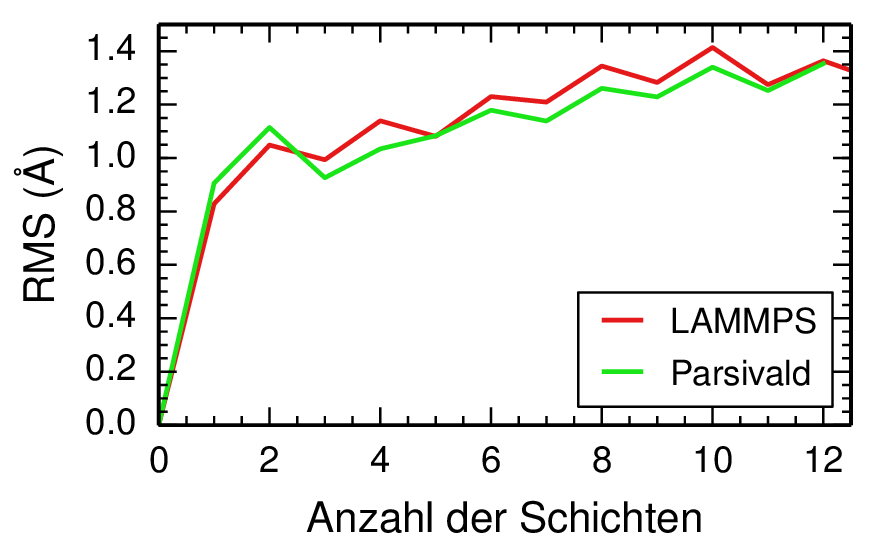
\includegraphics[width=\textwidth]{CuNi_layerroughness_comparison}
    \subcaption{
      Vergleich der Lagen-Rauheit (Abb.~\ref{fig:multilayerresults})
    }
    \label{fig:multilayerplots-a}
  \end{subfigure}
  \hfill
  \begin{subfigure}[t]{\subfigwidth}
    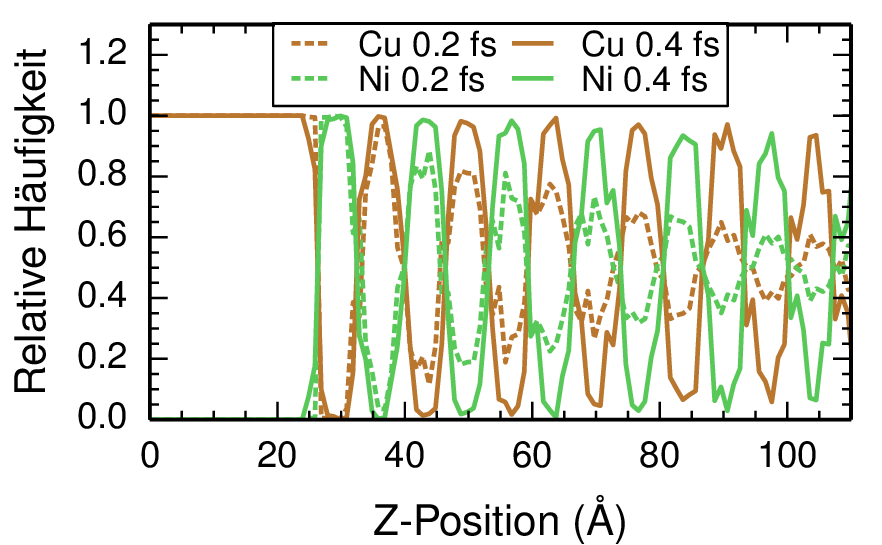
\includegraphics[width=\textwidth]{CuNi_atomdistribution_relax}
    \subcaption{Einfluss von $t_\text{relax}$ auf die Lagen-Qualität}
    \label{fig:multilayerplots-b}
  \end{subfigure}
  \caption[Rauheit und Qualität von Kupfer-Nickel-Multilagen]{
    Rauheit und Qualität von Kupfer-Nickel-Multilagen
  }
  \label{fig:multilayerplots}
\end{figure}

\begin{figure}
  \captionsetup[subfigure]{singlelinecheck=false}
  \def\subfigwidth{7cm}
  \begin{subfigure}[t]{\subfigwidth}
    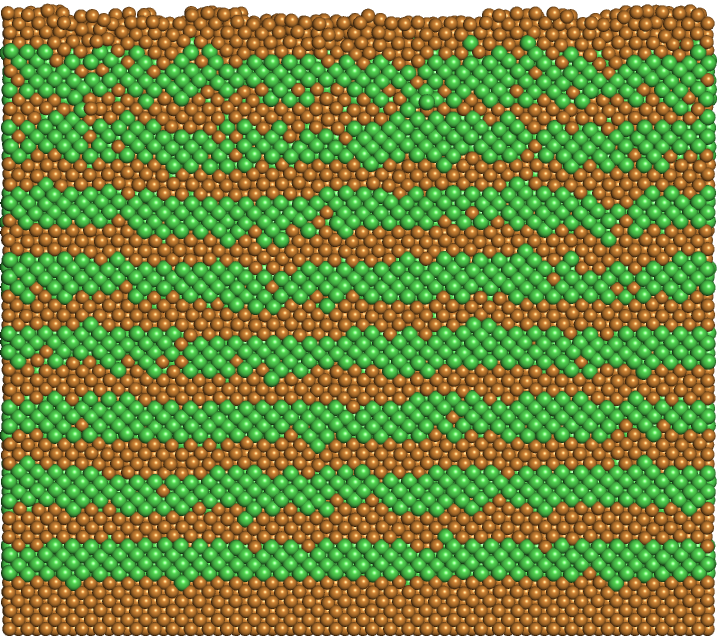
\includegraphics[width=\textwidth]{CuNi_profile_LAMMPS_nice}
    \subcaption{Profil von \ce{CuNi}-Multilagen mit LAMMPS}
  \end{subfigure}
  \hfill
  \begin{subfigure}[t]{\subfigwidth}
    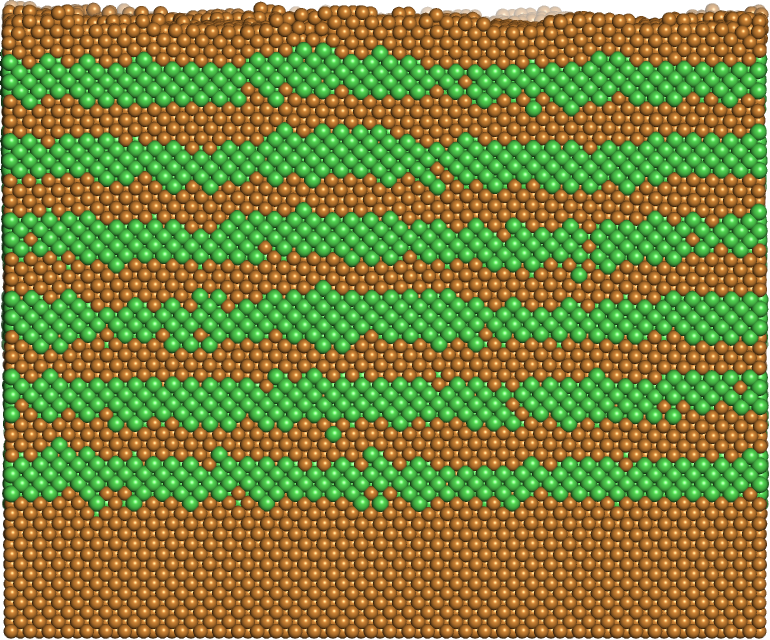
\includegraphics[width=\textwidth]{CuNi_profile_Parsivald}
    \subcaption{Profil von \ce{CuNi}-Multilagen mit Parsivald}
  \end{subfigure}
  \caption{Vergleich von Multilagen-Profilen mit LAMMPS und Parsivald}
  \label{fig:multilayerresults}
\end{figure}

\clearpage
\section{Silizium-PVD}
\label{siliconpvd}

Mit Silizium soll ein weiteres PVD-Material untersucht werden, das im Gegensatz zu den bisher untersuchten Metallen, welche ungerichtete Bindungen aufbauen und damit die kristalline Strukturen bevorzugen, auf gerichteten Bindungen beruht.
Deshalb werden reaktive Kraftfelder genutzt, welche auf einer expliziten Beschreibung gerichteter Bindungen über Bindungsordnungen benachbarter Atome basieren.

\subsection{Verfügbare ReaxFF-Parametrisierungen}

Da die ReaxFF-Formulierung erst innerhalb des letzten Jahrzehntes an Popularität gewonnen hat, sind die verfügbaren Potentiale auf sehr spezielle Probleme angepasst und unterstützen meist entweder Bulkmaterialien oder Reaktionen zwischen Molekülen.
Tabelle~\ref{tab:siliconpotentials} listet die im Rahmen der Arbeit untersuchten ReaxFF-Parametrisierungen auf, die in der Literatur gefunden werden konnten.

\begin{table}[hb]
  \caption{Untersuchte ReaxFF-Parametrisierungen für Silizium- und Siliziumoxidsysteme}
  \label{tab:siliconpotentials}
  \oddrowcolors
  \begin{tabularx}{1\textwidth}{|lXc|}
    \hline
    \textbf{Bezeichnung}  & \textbf{Anwendung \& Kommentare}                                                                          & \textbf{Ref.}                     \\
    \hline
    \pot{Al\_Al0\_AlN}    & \ce{Al}, \ce{Al2O3}, \ce{AlN}. Basiert auf einer Si-Parametrisierung                                      & \cite{plimpton_lammps_2014}       \\
    \pot{chenoweth}       & Zersetzung von Polydimethylsiloxane bei hohen Drücken und Temperaturen. Ergänzung von \ce{C-Si}-Bindungen & \cite{chenoweth_simulations_2005} \\
    \pot{kulkarni}        & Reaktion von Sauerstoff mit \ce{OH}-terminierten Siliziumoxid-Oberflächen                                 & \cite{kulkarni_oxygen_2013}       \\
    \pot{lg}              & ``low gradients''. Siehe liu\_nitramines. Fehlerhafte Version aus LAMMPS                                  & \cite{liu_reaxff-lg:_2011}        \\
    \pot{liu\_ettringite} & Verspannung von Ettringit (\ce{Ca6[Al(OH)6]2(SO4)3 26H2O}). Basiert auf Si-Parametrisierung               & \cite{liu_development_2012}       \\
    \pot{liu\_nitramines} & Dichtebestimmung von Nitramin-Molekülen bei hohen Drücken. Dichte erhöht durch Van-der-Waals-Korrekturen  & \cite{liu_reaxff-lg:_2011}        \\
    \pot{narayanan}       & Präparation mit \ce{Li-Al}-Silikaten. Für Phasenübergänge von Eukryptit-Kristallen (\ce{LiAl[SiO4]})      & \cite{narayanan_reactive_2012}    \\
    \pot{newsome}         & Oxidation von \ce{SiC}-Oberflächen mit \ce{O2} und \ce{H2O} bei \SIrange{500}{5000}{\kelvin}              & \cite{newsome_oxidation_2012}     \\
    \pot{nielson}         & Reaktionskinetik an Metallkatalysatoren bei hohen Temperaturen                                            & \cite{nielson_development_2005}   \\
    \pot{zhang}           & Zersetzung energetischer Moleküle (Nitramin-Explosionen)                                                  & \cite{zhang_carbon_2009}          \\
    \hline
  \end{tabularx}
\end{table}

\subsection{Voruntersuchungen}

In Ergänzung zu den bisherigen Voruntersuchungen, welche sich entsprechend der erwarteten Strukturen der abgeschiedenen Schichten auf die Beschreibung kristalliner Strukturen beschränkten, werden für die Silizium-Parametrisierungen auch die Eigenschaften amorpher Strukturen untersucht.
Die verwendeten Methoden wurden bereits in Abschnitt~\ref{mdmethods} vorgestellt.
Diese zusätzlichen Untersuchungen haben umfassendere Aussagen über die Anwendbarkeit der Parametrisierungen für vollständige Abscheidungssimulationen zum Ziel.
Die Ergebnisse dieser Betrachtungen sind in Tabelle~\ref{tab:siliconpreresults} zusammen gefasst und werden im Weiteren kurz diskutiert.

\begin{table}[th]
  \begin{threeparttable}
    \caption[Zusammenfassung der Voruntersuchungen für Silizium-Systeme]{
      Zusammenfassung der Voruntersuchungen für Silizium-Systeme.
      Siehe Anhang~\ref{appendix:silicon}
    }
    \label{tab:siliconpreresults}

    \oddrowcolors
    \begin{tabularx}{\textwidth}{|lCCCCCCC|}
      \hline
      \textbf{Bezeichnung}    & LMP\tnote{a} & c-\ce{Si} & c-\ce{SiO2} & a-\ce{Si} & \ce{SiH4} & \ce{+O2} & PVD\tnote{b} \\
      \hline                % & LAMMPS       & c-Si      & c-SiO2      & a-Si      & Silane    & +O2      & PVD          \\
      \pot{Al\_Al0\_AlN}      & \cmark       & ~         & (\cmark)    & \cmark    & \cmark    & ~        & \cmark       \\
      \pot{chenoweth}         & ~            & ~         & ~           & ~         & ~         & ~        & ~            \\
      \pot{kulkarni}          & \cmark       & \cmark    & \cmark      & \cmark    & \cmark    & (\cmark) & \cmark       \\
      \pot{lg}                & ~            & ~         & ~           & ~         & ~         & ~        & ~            \\
      \pot{liu\_ettringite}   & \cmark       & ~         & \cmark      & \cmark    & ~         & ~        & \cmark       \\
      \pot{liu\_nitramines}   & ~            & ~         & ~           & ~         & ~         & ~        & ~            \\
      \pot{narayanan}         & \cmark       & ~         & \cmark      & \cmark    & ~         & ~        & \cmark       \\
      \pot{newsome}           & \cmark       & ~         & (\cmark)    & ~         & ~         & (\cmark) & \cmark       \\
      \pot{nielson}           & \cmark       & \cmark    & \cmark      & \cmark    & \cmark    & ~        & \cmark       \\
      \pot{zhang}             & \cmark       & ~         & ~           & ~         & \cmark    & \cmark   & ~            \\
      \hline
    \end{tabularx}

 %% & CVD\tnote{b}
 %% & CVD
 %% & \cmark?
 %% & ~
 %% & \cmark?
 %% & ~
 %% & \cmark?
 %% & ~
 %% & \cmark?
 %% & \cmark?
 %% & \cmark?
 %% & ~

    \begin{tablenotes}[para]
      \item[a] LMP: Kompatibilität mit LAMMPS
      \item[b] PVD: a-\ce{Si}-PVD mit Parsivald
      %% \item[b] CVD: a-\ce{SiO2}-CVD mit Parsivald
    \end{tablenotes}
  \end{threeparttable}
\end{table}

\subsubsection{Kompatibilität mit der Molekulardynamiksoftware LAMMPS (LMP)}

Einige Potentialdateien sind aus unerfindlichen Gründen nicht mit der aktuellen Version der LAMMPS-Bibliothek kompatibel, was sich in harten Abbrüchen des Programmes äußert und sie von weiteren Untersuchungen ausschließt.
Andere Dateien lassen sich zwar laden und benutzen, äußern jedoch Warnungen über fehlerhafte van-der-Waals-Parameter, die aber nicht zu sonstigen Fehlern führen und meist nur Stickstoff- oder Platzhalteratome\footnote{ReaxFF-Parametrisierungen enthalten ein wechselwirkungsfreies Platzhalter-Element \ce{X} zum Zweck des Ausschlusses einzelner Atome aus der Simulation. Einige seiner Parameter werden von LAMMPS als fehlerhaft markiert.} betreffen.
Die Parametersätze \pot{chenoweth}, \pot{lg} und \pot{liu\_nitramines} können nicht mit LAMMPS genutzt werden.

\subsubsection{Kristalleigenschaften (c-\ce{Si}, c-\ce{SiO2})}

Diese Untersuchungen sind identisch zu den Untersuchungen der Kristallstrukturen aus den vorherigen Abschnitten.
Eine Parameterdatei gilt in dieser Hinsicht als erfolgreich, wenn eine Relaxierung der Kristallstruktur unterhalb der Schmelztemperatur von \SI{1687}{\kelvin}\cite{haynes_crc_2011} die Gittereigenschaften bewahrt, wofür die \todo{Diagramm mit den Dichten}Dichten und radialen Verteilungsfunktionen sowie die daraus gewonnenen \todo{Diagramm mit Koordinationszahlen und Bindungslängen}Koordinationszahlen und Bindungslängen verglichen werden.
Dabei überwiegen die Formen der radialen Verteilungsfunktionen, die nach dem langsamen Herunterkühlen der erhitzten Struktur wieder kristalline Eigenschaften zeigen sollten.
Dies geschieht allerdings nur bei \pot{kulkarni} und \pot{nielson}, wohingegen die anderen Parametrisierungen auch bei niedrigen \todo{wie niedrig waren die Experimente?}Temperaturen zu einer Verformung des Gitters hin zu amorphen Systemen neigen.
\todo{nicht auf Anhang verweisen?}\todo{vor allem: Informationen in den Anhang schreiben!}Detaillierte Informationen zu den Tests sind in Anhang~\ref{appendix_silicon} zu finden.

\subsubsection{Amorphes Silizium (a-\ce{Si})}

Durch langsame Relaxation zufällig positionierter Siliziumatome wurde amorphes Silizium generiert, das wie die Kristalle zuvor auf Dichte und Bindungslängen untersucht wurde.
Deren Werte variieren für amorphes Silizium stärker als für kristallines, liegen jedoch mit maximal \SI{4}{\percent} nah am experimentell bestimmten Wert für dünne Schichten von \SI{2.3}{\gpcc}\cite{remes_optical_1998}.
Die meisten Parametrisierungen erzeugen plausible Werte, wobei \pot{Al\_Al0\_AlN} und \pot{newsome} sehr starke Abweichungen zeigen.
Detaillierte Daten zu diesem Test sind in Anhang~\ref{appendix_silicon} zu finden.

\subsubsection{Abscheidungssimulationen (PVD)}

Die Simulationen von Silizium-PVD selbst verlaufen wie in Kapitel~\ref{parsivald} vorgestellt und unterscheiden sich kaum von den Parsivald-Simulationen der vorherigen Abschnitte.
Durch den Aufbau von gerichteten Bindungen zwischen den Silizium-Atomen wird die Bildung amorpher Schichten erwartet, die sich auch durch verringerte Mobilität der Atome auf der Oberfläche ergibt.
Eine Simulation gilt als erfolgreich, wenn die Parsivald-Simulation terminiert und einen dichten Silizium-Film gebildet hat, was nur bei \pot{newsome} nicht der Fall war\todo{was war bei newsome?}.

\subsection{Silizium-PVD}

\continuehere
Silizium-PVD dient in der Produktion elektronischer Bauelemente der Erzeugung einer dünnen, amorphen Siliziumschicht für unterschiedliche Anwendungsszenarien\todo{welche Anwendungen für a-Si? Solarzellen?}, für die konforme Schichten gleichbleibender Qualität gewünscht sind.
Durch den amorphen Charakter des Materials sind nanoskopische Leerstellen und höhere Rauheiten als bei monokristallinen Schichten zu erwarten, die im Folgenden kurz untersucht werden sollen.
\todo{Felix schreibt so was auch, wenn er keinen besseren Ausdruck findet.}Rechenaufwendigere Rechenvorschriften des ReaxFF-Potentiales legen eine längere Simulationsdauer als bei EAM-Potentialen nahe, weshalb nur eine kleine Menge an Simulationen durchgeführt wurde.
Typische Laufzeiten von mehreren Wochen wurden für vollständige ReaxFF-Abscheidungssimulationen beobachtet, jedoch sind im Gegensatz zu rein molekulardynamischen Untersuchungen größere Simulationsräume mit isolierten Ereignissen möglich, die eine Reduktion einiger Finite Size-Effekte zur Folge hat.

Als Substrat für die Parsivald-Simulationen wurden unrelaxierte Silizium-Monokristalle mit Oberflächen entlang der drei Kristallebenen (001), (011) und (111) präpariert und durch periodische Erweiterung auf \SI{106.416x103.68}{\angstrom} vergrößert.
Sonstige Parameter umfassen eine Temperatur von \SI{1300}{\kelvin} (der Schmelzpunkt liegt bei \SI{1687}{\kelvin}), Relaxationszeiten von \SI{350}{\femto\second} und MD-Box-Größen von \SI{37x37}{\angstrom}.
Die Auftreffenergie der Silizium-Atome liegt mit \SI{11.2}{\electronvolt} erneut vergleichsweise hoch, wird aber auch hier durch das Thermostat auf einen unbestimmten Wert verringert.
Damit werden im Schnitt \num{1.68} parallele Ereignisse mit durchschnittlich \num{1510.65} Atomen und einer mittleren Laufzeit von \SI{60.71}{\second} berechnet.
Die Laufzeit lässt sich beispielsweise über die Zeitschrittweite noch minimieren, zeigt allerdings den Unterschied in der Laufzeit bei der Nutzung von EAM- und ReaxFF-Potentialen, der einem Faktor von etwa \num{12} für vergleichbare Simulationen entspricht.
Die hohe Temperatur wurden zur Beschleunigung der Relaxationen gewählt und übersteigt die Temperaturen realer Abscheidungen.
Durch Optimierung der Simulation durch Relaxationszeit, Zeitschrittweite, Thermostatdämpfung und Teilchenenergie ließe sich die Temperatur auf einen realistischeren Wert bei gleicher Verlässlichkeit der Simulation senken.

Das Ergebnis der Abscheidungssimulation ist eine vergleichsweise glatte, amorphe Siliziumschicht, die mit konstanter Rate wächst, jedoch eine Zunahme der Rauheit aufgrund von sich langsam verstärkenden Oberflächenunebenheiten aufweist.

Zur Charakterisierung der Kristalleigenschaften der abgeschiedenen Schicht wurden ihre radiale Verteilungsfunktionen berechnet, aus denen ersichtlich ist, dass bereits nach \SI{4}{\angstrom}, also kurz vor der zweiten Korrelationslänge bei \SI{4.4}{\angstrom}, keine langreichweitige Ordnung mehr vorhanden ist.
Die engen Spitzen an den charakteristischen Abständen des reinen Silizium-Kristalles werden durch das Substrat erzeugt\todo{Schicht ohne Substrat RDF-untersuchen}, welches bei \SI{100}{\angstrom} Schichtdicke immerhin noch \SI{20}{\percent} der Struktur ausmacht, jedoch durch anfängliche Relaxierungen zum Teil seine Kristalleigenschaften verloren hat.
Anders als bei Gold oder Kupfer, bei denen metallische Bindungen dominieren, überwiegen in reinem Silizium kovalente Bindungen, so dass die mittleren Koordinationszahl von \num{3.99} anzeigt, dass alle 4 möglichen Bindungen der Siliziumatome tatsächlich ausgeprägt sind.
Somit zeigt sich die ReaxFF-Formulierung erfolgreich in der Darstellung der strukturellen Eigenschaften von Silizium.

\todoline{Anhang-Referenzen vermindern}
Die Unebenheiten der Schicht, welche die Form von Nanoporen annehmen, wachsen im Gegensatz zu den Kupfer-Kratern aus Abschnitt~\ref{copperpvd} mit der Oberfläche entlang der Wachstumsrichtung, schließen sich aber ebenfalls selbsttätig, wenngleich über einen größeren Zeitraum.
Abbildung~\ref{fig:siliconresults-a} stellt dazu über der Simulationszeit neben der Schichtdicke die Rauheit dar, welche im Verlauf der Simulation linear steigt und zuletzt einen RMS-Wert von \SI{1.15}{\nano\meter} annimmt, der experimentellen Erwartungen von \SIrange{1}{10}{\nano\meter} entspricht\cite{gago_nanopatterning_2002}.
An Abbildung~\ref{fig:siliconroughness} lässt sich erkennen, dass die Rauheit \todo{weiter schreiben}asd
\todo{Leider?}Leider ermöglicht die begrenzte Laufzeit der Simulation keine Aussage über den weiteren Verlauf der Rauheit, von der sublinearer Verlauf durch Schließung der Unebenheiten erwartet wird, wie er sich bei Sputterprozessen zeigt\cite{gago_nanopatterning_2002}\todo{Hinweis auf nicht-sublinearen Verlauf!}.

\begin{figure}
  \captionsetup[subfigure]{singlelinecheck=false}
  \def\subfigwidth{0.48\textwidth}
  \begin{subfigure}[t]{\subfigwidth}
    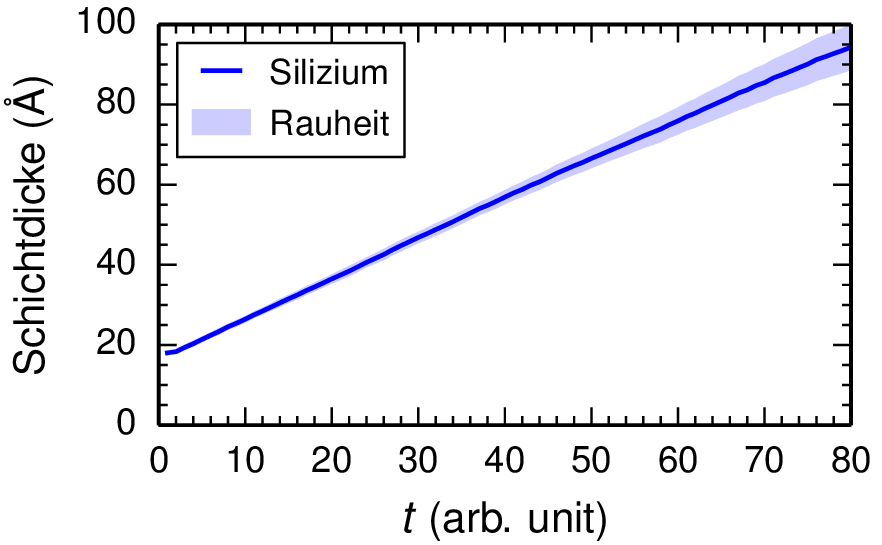
\includegraphics[width=\textwidth]{Si111_combined}
    \subcaption{Dicke und Rauheit der Schicht}
    \label{fig:siliconresults-a}
  \end{subfigure}
  \hfill
  \begin{subfigure}[t]{\subfigwidth}
    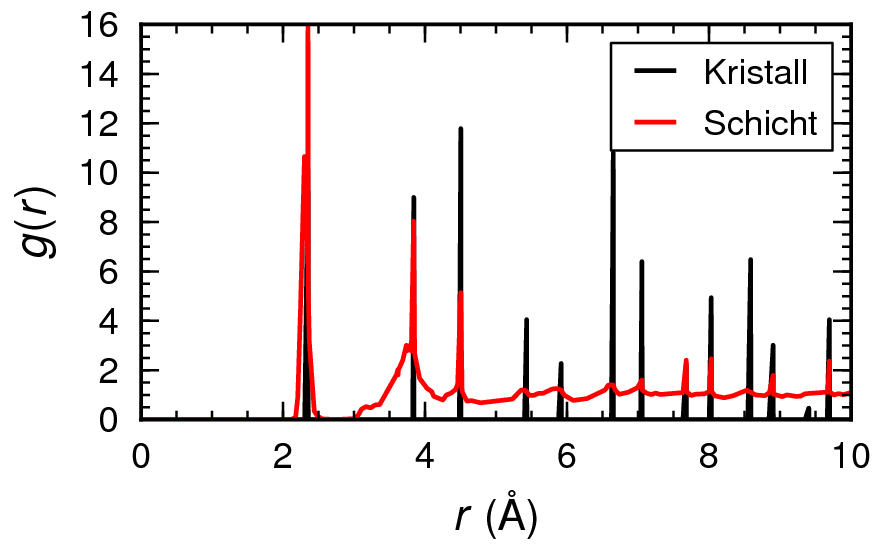
\includegraphics[width=\textwidth]{si111_rdf}
    \subcaption{Radiale Verteilungsfunktion bei $t=80$}
    \label{fig:siliconresults-b}
  \end{subfigure}
  \caption[Struktur einer Silizium-PVD-Schicht aus Parsivald]{
    Struktur einer Silizium-PVD-Schicht aus Parsivald (\SI{10x10}{\nano\meter})
  }
  \label{fig:siliconresults}
\end{figure}

Abbildung~\ref{fig:siliconprofile} stellt die räumliche Verteilung der Unebenheiten dar, die sich lokal in Kratern und Poren von bis zu \SI{32}{\angstrom} Tiefe konzentrieren, aufgrund ihrer geringen Breite aber nur zu einer RMS-Rauheit von \SI{11.5}{\angstrom} führen.
Breitere Krater haben sich durch die geringe Größe des Simulationsraumes nicht entwickelt, jedoch wäre eine Untersuchung einer ca. \SI{500x500}{\angstrom} breiten Struktur auf deren Bildung interessant.
Anhand des Profiles lässt sich auch erkennen, dass mitunter längere Relaxationszeiten oder höhere Teilchenenergien notwendig wären, um Porenbildung weiter zu verringern und langreichweitigere Unebenheiten zu befördern, wie sie etwa bei der Bildung nanoskopischer Silizium-Partikel auftreten würden.

Zum Vergleich beinhaltet Abbildung~\ref{fig:siliconunderrelaxedprofile} das Oberflächenprofil einer unterrelaxierten Oberfläche, wie sie während der Anpassung der Parsivald-Parameter entstanden sind.
Es zeigen sich stärkere Unterschiede und steilere Hänge, die sich aus der hohen Porösität des Materiales ergeben.
Die Porentiefen betragen \SI{6}{\nano\meter} und wachsen linear mit der Schichtdicke, wobei sich aus Zählung der Atome und des Volumens eine Dichte von \SI{2.634}{\gpcc} ergibt, welche durch die Unterschätzung der mittleren Höhe der Oberfläche durch die Nanoporen etwas überschätzt wird und somit oberhalb der kristallinen Dichte von \SI{2.32}{\gpcc} liegt.
Somit ist zu erwarten, dass die Rauheit der Schicht mit stärkerer Relaxierung während der Abscheidung weiter abnimmt.

\begin{figure}[H]
  \centering
  \captionsetup[subfigure]{singlelinecheck=false}
  \begin{subfigure}[t]{7.1cm}
    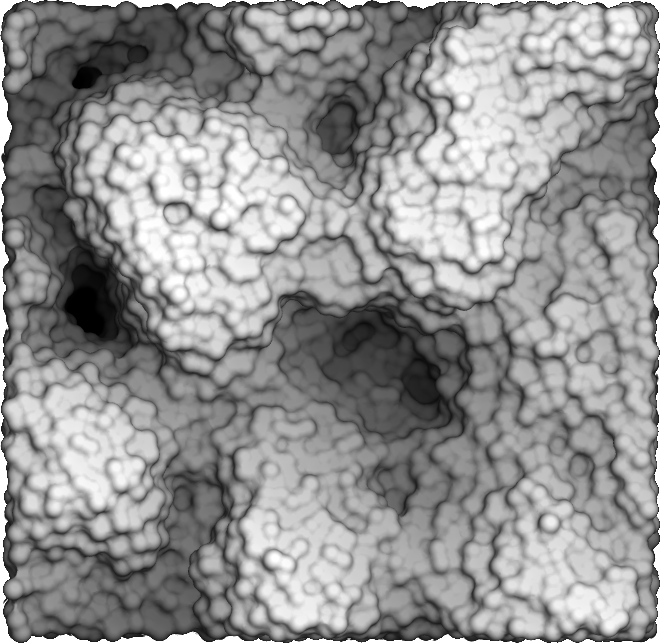
\includegraphics[width=\textwidth]{si111_surface_profile}
  \end{subfigure}
  \begin{subfigure}[t]{1.7cm}
    \def\svgwidth{\textwidth}
    \begin{overpic}[width=0.7cm]{greyhalfscale}
      \put(0,0){\input{img/si111_surface_profile_halfscale.pdf_tex}}
    \end{overpic}
  \end{subfigure}
  \caption[Oberflächenprofil einer Silizium-PVD-Schicht]{
    Oberflächenprofil einer auf Si-(111) per PVD abgeschiedenen Schicht
  }
  \label{fig:siliconprofile}
\todoline{Längenskala}
\end{figure}

\begin{figure}[H]
  \centering
  \captionsetup[subfigure]{singlelinecheck=false}
  \begin{subfigure}[t]{7.1cm}
    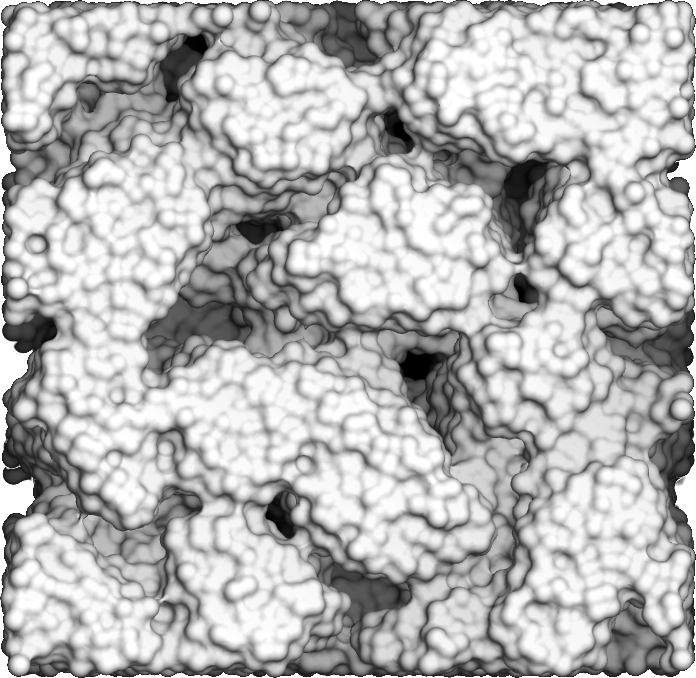
\includegraphics[width=\textwidth]{si111_underrelaxed_profile}
  \end{subfigure}
  \begin{subfigure}[t]{1.7cm}
    \def\svgwidth{\textwidth}
    \begin{overpic}[width=0.66cm]{greyscale}
      \put(0,0){\input{img/si111_underrelaxed_profile_scale.pdf_tex}}
    \end{overpic}
  \end{subfigure}
  \caption[Oberflächenprofil einer unterrelaxierten Siliziumschicht]{
    Oberflächenprofil einer unterrelaxierten, porösen Silizium-PVD-Schicht
  }
  \label{fig:siliconunderrelaxedprofile}
\end{figure}

\subsection{Voruntersuchungen für Siliziumdioxid-CVD}

ReaxFF-Potentiale versprechen die Simulation von Molekülen und deren Reaktion miteinander, die mit den folgenden Tests für Silan und molekularen Sauerstoff überprüft werden sollen.

\subsubsection{Stabilität der Precursormoleküle (\ce{SiH4}, \ce{O2})}

Simulationen einzelner und mehrerer Precursormoleküle (\ce{SiH4} und \ce{O2}) hinsichtlich ihrer Stabilität wurden im mikrokanonischen beziehungsweise kanonischen Ensemble bei verschiedenen Temperaturen durchgeführt.
\todo{Abbildung hier her kopieren}Abbildung~\ref{fig:silanestability} zeigt eine Auswahl der Ergebnisse der Silan-Simulationen, an denen sich erkennen lässt, wie instabile Simulationen zur Ablösung der Wasserstoffatome vom Silanmolekül führen.

\subsubsection{Reaktion der Precursormoleküle (\ce{SiH4 + O2})}

Reaktionen von einzelnen Precursormolekülen wurden stichprobenartig in verschiedenen Orientierungen, Energien und Temperaturen vorgenommen, um einen Überblick über die Verlässlichkeit zu bekommen.
Zusätzlich wurden durchmischte Precursorgase mit dem Ziel eventueller Reaktionen simuliert, was jedoch mit keiner der Parametrisierungen zum gewünschten Erfolg bei hoher Zuverlässigkeit führte.
Einige Parametrisierungen zeigen jedoch vielversprechende Teilreaktionen, die korrekte Doppelbindungen und Bildung von Wasserstoffmolekülen beinhalten (\todo{Abbildung hier her kopieren}Abbildung~\ref{fig:precursorreactions}).
Vor allem bei größeren Reaktionsräumen bilden sich Cluster aus Precursormolekülen, die von attraktiven Termen in den Kraftfeldern dominiert werden, aber nicht durch chemische Wechselwirkungen zu erklären sind (\todo{Abbildung hier her kopieren}Abbildung~\ref{fig:precursorclusters}).


\clearpage
\section{Aluminiumoxid-ALD}
\label{aluminaald}

Einen Vorzeige-Prozess für Atomlagenabscheidungen bildet die Abscheidung von Aluminiumoxid \ce{Al2O3}\cite{puurunen_surface_2005}, für die häufig das Precursorpaar Trimethylaluminium (TMA, \ce{Al(CH4)3}) und Wasser genutzt wird.
Mit einer Permittivität von $k\approx 8$ ersetzt Aluminiumoxid gemeinsam mit anderen Materialien langsam Siliziumdioxid ($k=3.9$) als Dielektrikum in der Halbleiterindustrie.
Deshalb soll der TMA-\ce{H2O}-Prozess im Folgenden besonders hinsichtlich der Reaktion der Precursormoleküle mit der Oberfläche untersucht werden.
Einige Reaktionen des Wasser-Halbzyklus' konnten dabei erfolgreich simuliert werden, wo hingegen die Simulation des TMA-Halbzyklus' bisher keinen Erfolg zeigte.

\subsection{Parametersätze}

Für die MD-Simulation von \ce{Al2O3} stehen drei Parametrisierungen zur Verfügung, die bereits aus den Untersuchungen der Silizium-Potentiale bekannt sind:\\
\textbf{Al\_AlO\_AlN} aus LAMMPS\cite{plimpton_lammps_2014}, \textbf{liu\_ettringite}\cite{liu_development_2012}, welches nachfolgend nur als \textbf{liu} geführt werden soll, und \textbf{narayanan}\cite{narayanan_reactive_2012}.
Ihnen ist gemein, dass sie ausgehend von Silizium-kompatiblen Potentialen um Parameter für Aluminium-Verbindungen erweitert wurden.
Auf eine Bewahrung der Konsistenz der Siliziumparameter wurde scheinbar verzichtet, so dass etwa mit der Liu-Datei eine verlässliche Simulation von  Silizium-Verbindungen verhindert, im Gegenzug aber die Simulation von Aluminium-Verbindungen ermöglicht wird.

Die Al\_AlO\_AlN-Datei stammt direkt aus der offiziellen LAMMPS-Distribution, wurde jedoch am 17. Mai 2013 nahezu kommentarlos aus dem Paket entfernt, was sich vermutlich auf mangelnde Kenntnis der Urheberschaft der Parameter sowie ihrer Zielsetzung zurückführen lässt.
Diese Vermutung wird von der Überarbeitung der Referenzen auf wissenschaftliche Publikationen für alle Parametersätze im selben Zeitraum gestützt.
Bei den Recherchen konnte kein Hinweis auf das ursprüngliche Anwendungsgebiet gefunden werden, weshalb mit diesen Parametern berechnete Eigenschaften gesondert überprüft werden sollten.
Es lässt sich jedoch sagen, dass es zeitgleich mit dem \textbf{lg}-Kraftfeld, welches sich bei den Silizium-Untersuchungen als unzureichend heraus gestellt hat, Eingang in LAMMPS gefunden hat.

Das Anwendungsgebiet der Liu-Potentialdatei liegt in der Simulation von Ettringit (\ce{Ca6[Al(OH)6]2(SO4)3 26H2O}), welches \ce{Al-O}-Bindungen und \ce{OH}-Gruppen enthält, so dass zumindest die Simulation des Bulkmateriales und einer hydroxylierten Oberfläche aussichtsreich erscheint.
Sie unterstützt einige der Precursorreaktionen und stellt sich daher als Favorit für Parsivald-Simulationen heraus, obwohl ihr eigentliches Anwendungsgebiet auf strukturellen Eigenschaften von Kristallen liegt.

Zuletzt steht die Narayanan-Parametrisierung für \ce{Li-Al}-Silikate für die Simulation von Eukryptit (\ce{LiAl[SiO4]}) zur Verfügung, lässt aber keine endgültige Aussage über die Qualität der \ce{Al-O}-Bindungen und \ce{OH}-Gruppen zu.
Zwar besteht ihr Trainingssatz aus verschiedenen Lithium-Aluminium-Kristallen, aber nur $\gamma$-\ce{LiAlO2} beinhaltet direkte \ce{Al-O}-Bindungen, wo hingegen keine der Strukturen Wasserstoff beinhaltet.
Es ist daher unwahrscheinlich, dass die Narayanan-Potentialdatei komplizierte Systeme verlässlich darstellt.

Abschließend lässt sich sagen, dass zur vollständigen Simulation der untersuchten Systeme die Erstellung einer eigenen Parametrisierung notwendig wäre, die jedoch den Fokus dieser Arbeit übersteigt.

\subsection{Voruntersuchungen}

Wie in den vorherigen Abschnitten werden hier separate Voruntersuchungen durchgeführt, zu denen die Reaktion von Precursormolekülen mit der Oberfläche ergänzt wurde.

\subsubsection{Strukturelle Eigenschaften von \ce{Al2O3}}

Zum Vergleich der strukturellen Eigenschaften des Bulkmateriales, wie etwa Dichte, Bindungslänge und Koordinationszahlen, wurde ein $\alpha$-\ce{Al2O3}-Kristall bei \SI{1500}{\kelvin} relaxiert und vor den abschließenden Messungen auf Raumtemperatur herunter gekühlt.
Durch einen methodischen Fehler wurden die Systeme zur Dichtebestimmung nicht vollends herunter gekühlt, weshalb die Referenzwerte anhand der Relaxationstemperatur korrigiert wurden.
Damit ergibt sich ein korrigierter Referenzwert zwischen \SI{3.95}{\gpcc} bei \SI{300}{\kelvin} und \SI{3.8}{\gpcc} bei \SI{1500}{\kelvin}\cite{fiquet_high-temperature_1999}, der im direkten Vergleich als \SI{3.85}{\gpcc} abgeschätzt wird.
Der dadurch entstehende Fehler ist im Vergleich zu Abweichungen um \SI{0.5}{\gpcc} gering.

Für die Bestimmung der Dichte der amorphen Struktur wurde das Bulkmaterial über den Schmelzpunkt von \SI{2317}{\kelvin} auf \SI{2555}{\kelvin} erhitzt, auf dieser Temperatur relaxiert und langsam auf Raumtemperatur abgekühlt.
Aufgrund der strukturellen Vielfalt bei amorphen Aluminiumoxiden lässt sich keine eindeutige Referenzdichte angeben, so dass auf den in diesem Zusammenhang häufig genannten Wertebereich von \SIrange{3.2}{3.6}{\gpcc} zurückgegriffen wurde.

Bindungslängen und Koordinationszahlen wurden direkt aus der radialen Verteilungsfunktion bestimmt, wobei die Referenzwerte auf gleiche Weise durch die Untersuchung der Kristallstruktur bestimmt wurden, welche mittels Materials Studio auf Basis eines $\alpha$-\ce{Al2O3}-Kristalles präpariert wurde.

\begin{table}
  \caption[Vergleich struktureller Eigenschaften von Bulk-\ce{Al2O3} mit verschiedenen Parametersätzen]{
    Vergleich struktureller Eigenschaften von Bulk-\ce{Al2O3} mit verschiedenen Parametersätzen.
    Bindungslängen und Koordinationszahlen stammen von einer relaxierten Kristallstruktur.
  }
  \label{tab:aluminabulks}

  \begin{tabularx}{\textwidth}{|Xllll|}
    \hline
    \textbf{Eigenschaft}    & \textbf{Referenz}    & \textbf{Al\_AlO\_AlN} & \textbf{liu}         & \textbf{narayanan}   \\
    \hline
    Dichte, amorph          & \SI{>3.2}{\gpcc}     & ~                     & \SI{3.66}{\gpcc}     & ~                    \\
    Dichte, kristallin      & \SI{3.85}{\gpcc}     & \SI{4.31}{\gpcc}      & \SI{3.88}{\gpcc}     & \SI{3.76}{\gpcc}     \\
    \ce{Al-O}-Bindungslänge & \SI{1.90}{\angstrom} & \SI{1.94}{\angstrom}  & \SI{1.88}{\angstrom} & \SI{1.85}{\angstrom} \\
    \ce{Al-O}-Koordination  & \num{4.00}           & \num{5.40}            & \num{4.55}           & \num{4.05}           \\
    \ce{Al-Al}-Koordination & \num{4.00}           & \num{6.66}            & \num{5.98}           & \num{5.10}           \\
    \ce{O-O}-Koordination   & \num{12.0}           & \num{12.4}            & \num{11.0}           & \num{12.2}           \\
    \hline
  \end{tabularx}
\end{table}

Die Ergebnisse dieser Untersuchungen (Tabelle~\ref{tab:aluminabulks}) zeichnen ein vielseitiges Bild.
Einerseits stimmen die Bindungslängen für alle Parametrisierungen auf \SI{2}{\percent} überein, andererseits ergeben sich aber große Unterschiede in der Dichte der Kristalle, die sich nicht mit den Bindungslängen korreliert sind.

So liegt für die Al\_AlO\_AlN-Parameter eine Abweichung um \SI{+12}{\percent} in der Dichte vor, allerdings ist die Bindungslänge um \SI{2}{\percent} erhöht, was für ähnliche Strukturen zu einer Ausdehnung des Kristalles und somit eine Verringerung der Dichte um \SI{6}{\percent} führen müsste.
Erst bei Betrachtung der Koordinationszahlen zeigt sich die Ursache der Abweichung, die mit einer \ce{Al-O}-Koordinationszahl von \num{5.4} (Kristall: \num{4.0}) in einer Verformung des Kristalles liegt.
Da $\alpha$-\ce{Al2O3} mit \SI{3.95}{\gpcc} eigentlich die dichteste Phase bei Normaldruck ist, sollten nur Übergänge zu weniger dichten Konfigurationen wie amorphem Aluminiumoxid oder etwa $\gamma$-\ce{Al2O3} möglich sein, das aufgrund seiner Porösität eine geringere Dichte von etwa \SI{3.67}{\gpcc}\cite{dynys_alpha_1982} aufweist.
Da hier das Gegenteil der Fall ist, wurde die Al\_AlO\_AlN-Parameterdatei in vielen der nachfolgenden Untersuchungen nicht weiter betrachtet.

Die Liu-Parametrisierung weist ebenfalls eine geringe Änderung aller Koordinationszahlen auf, die sich in einer nur minimalen Verringerung der Dichte äußert.
Anhand einer \ce{Al}-{O}-Koordination von \num{4.55} ist ersichtlich, dass die $\alpha$-Phase mit diesem Parametersatz nicht stabil ist und stattdessen scheinbar eine vergleichsweise dichte amorphe Phase angenommen wird.
Für diesen Parametersatz wurde deshalb auch die Dichte eines amorphen Materiales mit \SI{3.66}{\gpcc} bestimmt, die zwar innerhalb des üblicherweise für amorphe Materialien genannten Bereiches von \SIrange{3.2}{3.6}{\gpcc} liegt, ansonsten aber unterhalb der im ersten Schritt bestimmten Dichte liegt, womit eine höhere Porösität denkbar wird.

Zum Schluss zeigt Die Narayanan-Parameterdatei die besten Ergebnisse für kristalline Strukturen, obwohl sowohl die Bindungslänge als auch die Dichte ca. \SI{2}{\percent} unterhalb der jeweiligen Referenzwerte liegen.
Dies ist im Zusammenhang mit dem Fehlen von \ce{Al-O}-Bindungen in den meisten Molekülen des Trainingssatzes eher überraschend, zeigt aber die Orthogonalität der einzelnen ReaxFF-Parameter, da so die Eigenschaften von $\gamma$-\ce{LiAlO2} die \ce{Al-O}-Bindungen dominieren, statt beim Fitting überschrieben zu werden.

\subsubsection{Precursor-Simulationen}

Zur Untersuchung der Stabilität der Precursor wurden diese einzeln präpariert und per LAMMPS mit verschiedenen Kraftfeldern im kanonischen Ensemble simuliert.
Dabei war schnell ersichtlich, dass Trimethylaluminium (TMA) von der Liu- sowie der Narayanan-Parametrisierung in Ermangelung der Ausprägung von \ce{Al-C}-Bindungen praktisch nicht simuliert werden kann.
Die Methylgruppen binden nicht mit dem zentralen Aluminium-Atom, so dass sie sich von diesem mit fortlaufender Simulationszeit linear entfernen.
Einzig mittels des bereits ausgeschlossenen Al\_AlO\_AlN-Parametersatzes lassen sich stabile TMA-Moleküle simulieren.

\todo[inline]{Bilder im Anhang}

Simulationen von Wassermolekülen sind hingegen mit allen Parametrisierungen geglückt, doch wurden keine umfangreicheren Untersuchungen etwa hinsichtlich der Phasenübergänge angestellt.
Anhand des Al\_AlO\_AlN-Parametersatzes wurden auch Reaktionen zwischen TMA und Wasser simuliert, wie sie beispielsweise bei Vermischung der Precursorgase im ALD-Reaktor auftreten können, aber \todo{phrasing}leider ohne Erfolg.
Es zeigt sich, dass die \ce{Al-C}-Bindungen entweder zu stark oder in zu großem Maß von den Methylgruppen abgeschirmt sind.

\subsubsection{Precursor-Oberflächen-Reaktionen}

Anstatt die Precursormoleküle in der Gasphase reagieren zu lassen, werden hier einzelne Wassermoleküle auf eine $\alpha$-\ce{Al2O3}-Kristalloberfläche gebracht, die mit den darauf befindlichen Sauerstoffatomen reagieren und die Oberfläche so hydroxylieren sollen\todo{Ref}.
Zu diesem Zweck wurde ein mehrschichtiges System mit einem kristallinen Substrat und einer Schicht von Wassermolekülen in Gasphase präpariert, wie es in Abbildung~\ref{fig:wateraluminasurface-a} dargestellt ist.
In der Simulation werden die Wassermoleküle mit einer maxwellschen Geschwindigkeit entsprechend \SI{500}{\kelvin} versehen, die Atome an der Unterseite des Substrates fest gehalten und das Berendsen-Thermostat auf den verbleibenden Teil des Substrates angewandt.
Damit handelt es sich zwar streng gesehen nicht mehr um eine Simulation im kanonischen Ensemble, aber man verzichtet auf separate Integratoren für Substrat (NVT) und Wasser (NVE), deren Grenzen bei erfolgreichen Reaktionen ohnehin aufgelöst werden.

\begin{figure}
  \captionsetup[subfigure]{singlelinecheck=false}
  \def\subfigwidth{0.32\textwidth}
  \begin{subfigure}[t]{\subfigwidth}
    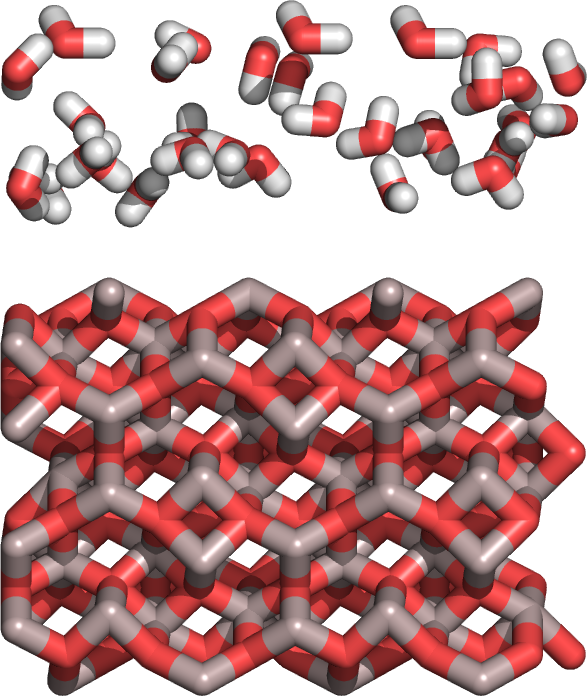
\includegraphics[width=\textwidth]{alumina_h2o_before}
    \subcaption{Seitenansicht, vorher}
    \label{fig:wateraluminasurface-a}
  \end{subfigure}
  \hfill
  \begin{subfigure}[t]{\subfigwidth}
    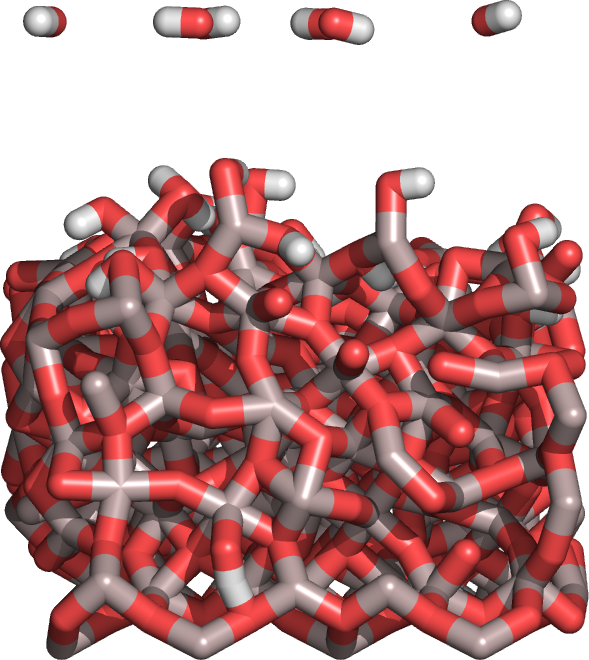
\includegraphics[width=\textwidth]{alumina_h2o_after}
    \subcaption{Seitenansicht, nachher}
    \label{fig:wateraluminasurface-b}
  \end{subfigure}
  \hfill
  \begin{subfigure}[t]{\subfigwidth}
    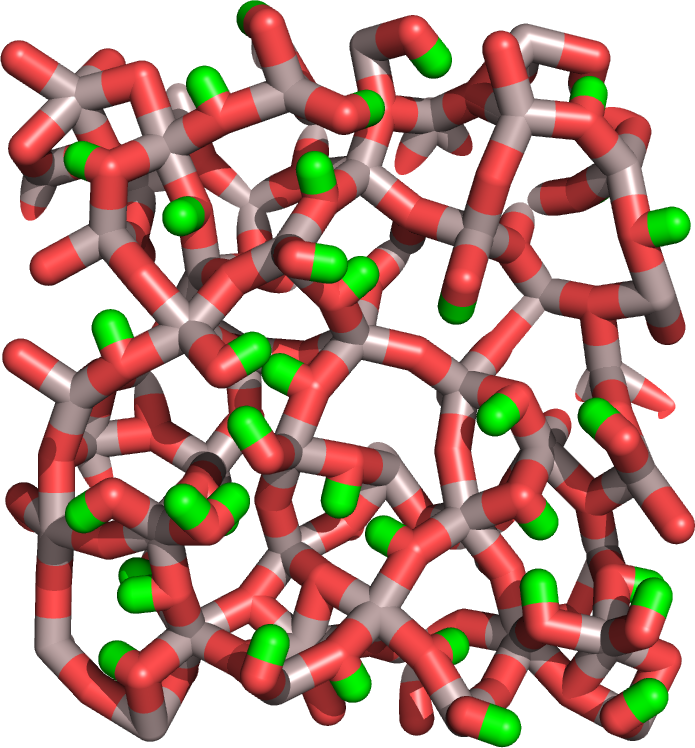
\includegraphics[width=\textwidth]{alumina_h2o_topview}
    \subcaption{Draufsicht, nachher.
      Hydroxyl ist grün hervorgehoben.
    }
    \label{fig:wateraluminasurface-c}
  \end{subfigure}
  \caption[Oberflächenreaktion von Wasser mit $\alpha$-\ce{Al2O3}]{Ergebnisse einer Oberflächenreaktion von Wasser mit $\alpha$-\ce{Al2O3}.
    Das Wasser reagiert mit Sauerstoffatomen an der Oberfläche zu Hydroxylgruppen.
  }
  \label{fig:wateraluminasurface}
\end{figure}

Das Ergebnis der Simulationen für die Liu-Parameter (Abbildungen~\ref{fig:wateraluminasurface-b} und~\ref{fig:wateraluminasurface-c}) zeigt die gleichmäßige Bedeckung der Oberfläche mit Hydroxylgruppen (\SI{9.5}{\per\square\nano\meter}) neben gelegentlich adsorbierten Wassermolekülen, die keine Oberflächenreaktion eingegangen sind.
Letztere sollten aber auf längere Sicht durch die Einflüsse der Überkoordinationsterme des ReaxFF-Potentiales entweder zerfallen oder sich von der Oberfläche lösen.
Trotz unterschiedlicher Startbedingungen stimmt der maximale Bedeckungsgrad der Oberfläche mit Hydroxylgruppen mit aus Elektronenstrukturrechnungen bestimmten Maximalwerten von \SI{9.2}{\per\square\nano\meter}\cite{kim_energy_2011} überein.
Zu Beginn der Simulationen wurden ausreichende Mengen von Wassermolekülen für Bedeckungsgrade von \SI{5.8}{\per\square\nano\meter}, \SI{19.0}{\per\square\nano\meter} und \SI{57.6}{\per\square\nano\meter} präpariert, von denen die überschüssigen Wasser-Moleküle nicht mit der Oberfläche binden, sondern in der Gasphase verbleiben, wie in Abbildung~\ref{fig:wateraluminasurface-b} am oberen Rand des periodischen Simulationsraumes erkennbar ist.
Einige der Wassermoleküle sind durch periodische Randbedingungen des Simulationsraumes zerteilt, weshalb es sich scheinbar um Hydroxylmoleküle handelt, tatsächlich aber komplette Wassermoleküle verbleiben.
Es zeigt sich also die sterische Hinderung der Wasserstoffmoleküle gegenüber weiteren Reaktionen von Wasser mit der Oberfläche.

Eine repulsive Kraft zwischen den Wassermolekülen und der Oberfläche verhindert diese Reaktionen unter Nutzung der Narayanan-Parameter.
Das deutet darauf hin, dass Hydroxylgruppen auf einer Aluminiumoxid-Oberfläche energetisch nicht bevorzugt werden oder die Reaktion mit einer hohen Reaktionsbarriere verbunden ist.
Zusammen mit dem Problem, Trimethylaluminium nicht darstellen zu können, ist dieser Parametersatz somit nicht in der Lage, den ALD-Prozess darzustellen.

\todo[inline]{Hinweis auf vollständige ALD-Simulationen?}
\todo[inline]{Welche der alten Ergebnisse finden hier Anwendung?}

